\chapter{Heat, Navier Stokes and Schr\"odinger: Examples and Experiments}
\label{ch:examples}

\section{Worked example: the heat equation}\label{m:sec:heat}

Chapters~\ref{ch:manifold} to~\ref{ch:generators} state the method, generative Bayesian computation (GBC), and its theory for a general evolution equation. This chapter puts three equations through them and asks what the theorems say about each and what an implementation delivers. It assumes from Chapter~\ref{ch:manifold} the observation model, the Bernstein von Mises theorems of Nickl and of Konen and Nickl with Conditions 1 and 2 of Nickl on the prior and the forward map, and Algorithm~\ref{m:alg:gbc}; from Chapter~\ref{ch:adjoint} the adjoint summary and the dimension $J_N$ that the theory licenses for it; and from Chapter~\ref{ch:generators} the transfer theorem, the accuracy it asks of a generator, and the localized training of Algorithm~\ref{m:alg:loc}. A result there that is conditional on Assumption~\ref{m:ass:U} or Assumption~\ref{m:ass:u2p} is conditional here in the same way: the first is open (Open Question~\ref{m:op:unif}), and the second holds in the setting of Theorem~\ref{m:thm:u2ploc}.

The heat equation comes first because every object in it is explicit. Two dimensional Navier Stokes about the Taylor Green vortex adds the nonlinearity as a compact correction to the heat equation case. The Schr\"odinger equation removes the dissipation, and with it the smoothing on which the supremum norm theorems rest. The last two sections connect the construction to earlier methods that share its structure and to the sixth problem, and list five questions that remain open. Except where a result is attributed, the computations and experiments are ours, and the Notes at the end say which results are quoted and which are, to our knowledge, new.

Let $\Omega=\T^d$, $\partial_tu=\nu\Delta u$, $u(0)=\theta$, so that $u_\theta(t,x)=\sum_j e^{-\nu\lambda_jt}\theta_je_j(x)$ with $\lambda_j=4\pi^2|k_j|^2$. Take the prior $\theta_j\sim N(0,\rho^2\lambda_j^{-\alpha})$ independently, truncated to $|k|\le K_{\max}$, and observations \eqref{m:eq:model} with $t_i\sim\mathrm{Unif}[T_0,T]$, $x_i\sim\mathrm{Unif}(\T^d)$.

\subsubsection{Exact posterior and sufficient statistic} By \eqref{m:eq:linpost}, the posterior is $N(m_N,V_N)$ with $V_N^{-1}=\Phi^\top\Phi+\rho^{-2}\Lambda^\alpha$, and the sufficient statistic is $S_N=\Phi^\top Y$, i.e.\ $S_{N,j}=\sum_ie^{-\nu\lambda_jt_i}e_j(x_i)Y_i$: the data projected onto mode $j$ and propagated backward by the (self adjoint) heat semigroup to time zero.

\subsubsection{Information per mode and the dissipation barrier} By \eqref{m:eq:gram},
\begin{equation}\label{m:eq:iota}
\begin{aligned}
\frac1N\Phi^\top\Phi&\to\diag(\iota_j),\\
\iota_j(T_0)&=\frac{1}{T-T_0}\int_{T_0}^Te^{-2\nu\lambda_jt}dt\\
&=\frac{e^{-2\nu\lambda_jT_0}\big(1-e^{-2\nu\lambda_j(T-T_0)}\big)}{2\nu\lambda_j(T-T_0)} .
\end{aligned}
\end{equation}
With $T_0=0$, $\iota_j\asymp(2\nu\lambda_jT)^{-1}$ decays polynomially in $j$; with $T_0>0$ the factor $e^{-2\nu\lambda_jT_0}$ makes it decay exponentially in $|k_j|^2$. Table~\ref{m:tab:iota} gives the values and Figure~\ref{m:fig:heat}(left) plots them. At $|k|=16$ the information drops by a factor of about $2\times10^4$ when the first observation is delayed to $T_0=0.05$, and by about $10^{17}$ at $T_0=0.2$. This is the mechanism of the inverse logarithmic lower bound in Theorem~4 of Nickl and Titi~\cite{nickltiti2024}, as a table: a mode that has decayed by $e^{-\nu\lambda_jT_0}$ before the first observation is recoverable only with about $e^{2\nu\lambda_jT_0}$ times more data, the square of that factor, since the information a mode carries scales with the square of its amplitude. It is also the viscous curse in the computation of Nickl and Wang~\cite{nicklwang2024} (Section~\ref{sec:gradstab}). Were their remaining conditions to carry over, the curvature constant $c_{\min}$ of their localized Langevin algorithm would be $\min_j\iota_j$, which Section~\ref{m:sec:nondiss} contrasts with the dispersive case, where it is one uniformly.

\begin{table}[t]\centering\small
\caption{Per mode information $\iota_k(T_0)$ for the two dimensional heat equation, $\nu=0.01$, $T=1$, mode $k=(|k|,0)$. Here $T_0$ is the time at which observation begins, so that $T_0=0$ is the design of \eqref{m:eq:model} and $T_0>0$ delays the start; the closed form is \eqref{m:eq:iota}.}\label{m:tab:iota}
\begin{tabular}{rllll}
\toprule
$|k|$ & $\iota_k(0)$ & $\iota_k(0.05)$ & $\iota_k(0.2)$ & $1/\iota_k(0)=\sigma_k^2$\\
\midrule
1 & $6.91\times10^{-1}$ & $6.76\times10^{-1}$ & $6.33\times10^{-1}$ & $1.45$\\
2 & $3.03\times10^{-1}$ & $2.70\times10^{-1}$ & $1.94\times10^{-1}$ & $3.30$\\
4 & $7.92\times10^{-2}$ & $4.43\times10^{-2}$ & $7.91\times10^{-3}$ & $12.6$\\
8 & $1.98\times10^{-2}$ & $1.66\times10^{-3}$ & $1.01\times10^{-6}$ & $50.5$\\
16 & $4.95\times10^{-3}$ & $2.13\times10^{-7}$ & $1.72\times10^{-20}$ & $202$\\
32 & $1.24\times10^{-3}$ & $3.61\times10^{-21}$ & $9.17\times10^{-74}$ & $809$\\
\bottomrule
\end{tabular}
\end{table}

\begin{figure}[tp]\centering
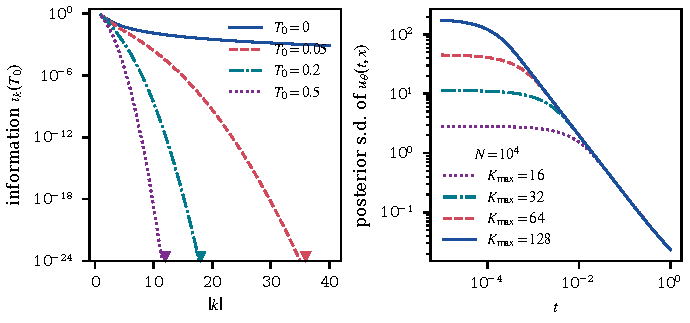
\includegraphics[width=\textwidth]{mf_heat}
\caption{Left: per mode information $\iota_k(T_0)$ from \eqref{m:eq:iota} for the two dimensional heat (Stokes) equation, $\nu=0.01$, $T=1$, for four observation start times; a triangle marks where a curve falls below $10^{-24}$ and leaves the frame. Right: posterior standard deviation of $u_\theta(t,x)$ at a fixed point, $\sqrt{\sum_{0<|k|\le K_{\max}}e^{-2\nu\lambda_kt}/(N\iota_k)}$ with $\iota_k=\iota_k(0)$, as a function of $t$ for $N=10^4$ and four truncations, $K_{\max}=16,32,64,128$. The $1/\sqrt N$ scaling is exact. At each fixed truncation the sum is finite at $t=0$ and the curve ends in a plateau, which rises by a factor close to four each time $K_{\max}$ doubles and so grows without bound with the truncation: this divergence as $t\to0$ is the failure of the supremum norm Bernstein von Mises theorem at the initial time. For larger $t$ the curves coincide, and the finiteness of the sum there whatever the truncation is parabolic smoothing.}\label{m:fig:heat}
\end{figure}

\begin{proposition}[Gram concentration and the finite $N$ Bernstein von Mises error]\label{m:prop:gram}
Let $\Phi$ be the design matrix \eqref{m:eq:design} for the heat equation with $D$ modes, uniform design on $[0,T]\times\T^d$, and $\norm{e_j}_\infty\le\sqrt2$, and let $N\ge D\log D$. Then, with the absolute constant $c=12$,
\[
\begin{gathered}
\Big\|\frac1N\Phi^\top\Phi-\diag(\iota_j)\Big\|_{op}\le c\,\sqrt{\frac{D\log D}{N}}\\
\text{with probability at least }1-D^{-1},
\end{gathered}
\]
and consequently, if $c\sqrt{D\log D/N}<\min_j\iota_j$, for the exact posterior covariance $V_N=(\Phi^\top\Phi+\Sigma_0^{-1})^{-1}$ and its Bernstein von Mises prediction $\bar V_N=(N\diag(\iota_j)+\Sigma_0^{-1})^{-1}$,
\[
\begin{gathered}
\norm{NV_N-N\bar V_N}_{op}\le\frac{c\sqrt{D\log D/N}}{\min_j\iota_j\,(\min_j\iota_j-c\sqrt{D\log D/N})}\\
\text{on the same event.}
\end{gathered}
\]
\end{proposition}

\begin{proof}
$\frac1N\Phi^\top\Phi=\frac1N\sum_i\phi_i\phi_i^\top$ with $\phi_i=(s_j(t_i)e_j(x_i))_j$ i.i.d., $E\phi_i\phi_i^\top=\diag(\iota_j)$ by orthonormality of $(e_j)$ and \eqref{m:eq:iota}, and $\norm{\phi_i}^2\le2D$. The matrix Bernstein inequality~\cite[Theorem 6.1.1]{tropp2015}, applied to the centered summands $(\phi_i\phi_i^\top-\diag(\iota_j))/N$, whose operator norms are at most $L=4D/N$ and whose variance proxy is at most $v=2D\max_j\iota_j/N\le2D/N$, bounds the probability that $\norm{N^{-1}\Phi^\top\Phi-\diag(\iota_j)}_{op}\ge t$ by $2D\exp\{-(t^2/2)/(v+Lt/3)\}$. At $t=\frac23\ell L+\sqrt{2\ell v}$ with $\ell=\log(2D^2)$ the exponent is at least $\ell$, so this probability is at most $D^{-1}$. For $D\ge2$, $\ell\le3\log D$, hence $t\le8D\log D/N+\sqrt{12D\log D/N}\le(8+\sqrt{12})\sqrt{D\log D/N}<12\sqrt{D\log D/N}$, where the middle step uses $D\log D/N\le1$; for $D=1$ the probability claimed is $0$ and there is nothing to prove. The second follows from the resolvent identity $NV_N-N\bar V_N=N\bar V_N(N\diag\iota-\Phi^\top\Phi)V_N$ and $\norm{N\bar V_N}_{op}\le1/\min_j\iota_j$, $\norm{NV_N}_{op}\le(\min_j\iota_j-c\sqrt{D\log D/N})^{-1}$.
\end{proof}

Since $\min_{j\le D}\iota_j\asymp D^{-2/d}$ by \eqref{m:eq:iota}, the relative error of the Bernstein von Mises covariance is $O(D^{2/d}\sqrt{D\log D/N})$, which is small exactly when $D\ll N^{d/(d+4)}$ up to logarithms. This is a quantitative counterpart, for the linear problem, of the dimension $J_N\asymp N^{d/(2\gamma+d)}$ of the projection $p_N$ in Nickl's centering \eqref{m:eq:thetahat} (his prior \eqref{m:eq:prior} is not truncated, and Condition~1 of Nickl~\cite{nicklbvm2024} imposes no dimension constraint).

\subsubsection{The Bernstein von Mises theorem, checked at finite $N$} Theorem~\ref{m:thm:nickl2} predicts that the posterior on mode $j$ is asymptotically $N(\tilde\theta_j,\sigma_j^2/N)$ with $\sigma_j^2=1/\iota_j$, and more precisely, keeping the prior term, with variance $(N\iota_j+\rho^{-2}\lambda_j^\alpha)^{-1}$. Figure~\ref{m:fig:heatgbc} compares this with the exact posterior from \eqref{m:eq:linpost} for the fixed truth $\theta_{0,k}=(1+k^2)^{-1}\mathrm{sign}(\sin k)$: the maximal relative discrepancy between the exact and the asymptotic standard deviation is $1.4\times10^{-4}$. The limit $\Ncal_{\theta_0}$ has variance $\sigma_j^2\asymp2\nu\lambda_jT$ growing with $j$, so $\sum_j\lambda_j^{-a}\sigma_j^2<\infty$ exactly when $a>1+d/2$, which is the tightness range of Proposition~2 of Nickl~\cite{nicklbvm2024}; the Gaussian limit is white noise roughened by $(-\Delta)^{1/2}$, and lives in $H^{-a}$ but not in $L^2$.

\begin{figure}[tp]\centering
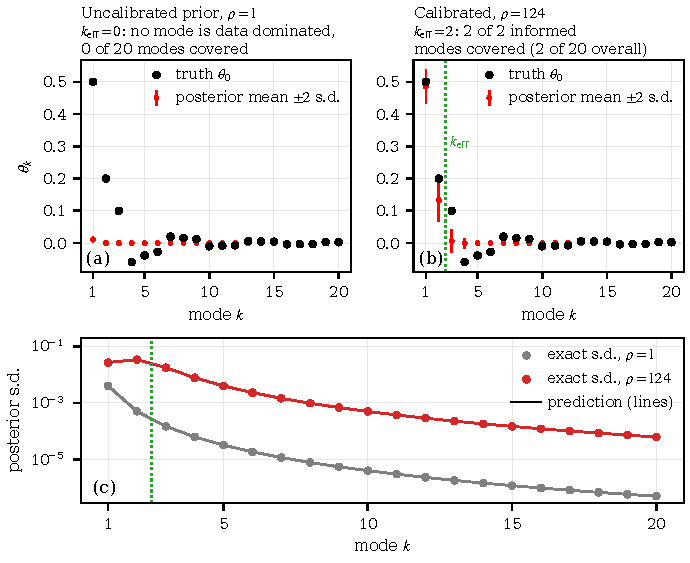
\includegraphics[width=\textwidth]{mf_heat_gbc}
\caption{Heat equation on $\T^1$, $N=2000$ observations, $K_{\max}=20$, $\alpha=3$, $\nu=0.01$, with the exact posterior of \eqref{m:eq:linpost}. Panel (a): the uncalibrated prior, $\rho=1$. No mode is data dominated, $k_{\rm eff}=0$; the truth lies up to $4949$ prior standard deviations from the prior mean and outside a two standard deviation credible interval in all $20$ modes. Panel (b): the same data with $\rho$ calibrated so that the prior standard deviation at $|k|=1$ matches the initial condition, $\rho=124$. Now $k_{\rm eff}=2$, and the truth lies inside the interval in every informed mode, with largest standardized error $1.96$. Panel (c): exact posterior standard deviation per mode in both settings against the prediction $(N\iota_k+\rho^{-2}\lambda_k^\alpha)^{-1/2}$ (lines). The agreement is close in both, which is why it validates nothing for $\rho=1$. Section~\ref{m:sec:expfinite} gives the diagnosis and Section~\ref{m:sec:covstudy} the coverage over replicates.}\label{m:fig:heatgbc}
\end{figure}

\subsubsection{Forward simulation and the trajectory theorem} Pushing the posterior through the heat flow gives $u_\theta(t,x)\mid Z\sim N\big(\sum_je^{-\nu\lambda_jt}\tilde\theta_je_j(x),\ \sum_{j,l}e^{-\nu(\lambda_j+\lambda_l)t}(V_N)_{jl}e_j(x)e_l(x)\big)$. Keeping only the diagonal terms, which is justified asymptotically because $\frac1N\Phi^\top\Phi$ concentrates on $\diag(\iota_j)$ by Proposition~\ref{m:prop:gram}, the posterior standard deviation of the state at time $t$ is, asymptotically, $N^{-1/2}\big(\sum_je^{-2\nu\lambda_jt}\sigma_j^2e_j(x)^2\big)^{1/2}$. Since $\sigma_j^2\asymp\lambda_j$, the series $\sum_j\lambda_je^{-2\nu\lambda_jt}$ converges for every $t>0$ and diverges at $t=0$: the trajectory is $\sqrt N$ estimable in supremum norm at every positive time, and the initial condition is not. Figure~\ref{m:fig:heat}(right) shows this, which is Theorem~\ref{m:thm:nickl1} and Remark~3 of Nickl~\cite{nicklbvm2024} in one picture; it is also Corollary~\ref{m:cor:commute}, since for a linear equation solve then simulate and simulate the limit are the same operation.

\subsubsection{GBC for the heat equation} Algorithm~\ref{m:alg:gbc} with the preconditioned summary $\tilde S_N=V_N\Phi^\top Y$ of Proposition~\ref{m:prop:linsuff} and an identity plus scale generator is exact. The learning problem has $D$ slopes (all equal to one), $D$ intercepts (all zero) and a $D\times D$ scale; with the prior diagonal and the Gram matrix asymptotically diagonal, the scale is asymptotically diagonal with entries $(N\iota_j+\rho^{-2}\lambda_j^\alpha)^{-1/2}$, so a generator with an identity skip, which fixes the slopes, and $2D$ free parameters, the intercepts and the diagonal of the scale, suffices, and $M\gg D$ simulations estimate it. This is the baseline against which the nonlinear case should be measured: the cost of nonlinearity is exactly the cost of the compact perturbation $\Kcal$ in \eqref{m:eq:fredholm}.

\subsection{The resolution the data support}\label{m:sec:resolution}

Four truncation dimensions appear in this part and they are different objects, so we fix them here once, in Table~\ref{m:tab:dims}.

\begin{table}[t]\centering\small
\caption{The four truncation dimensions, with the values they take in the computations of this part. The last column reports what is actually used, over $N=10^3$ to $1.3\times10^6$ where a range is given.}\label{m:tab:dims}
\begin{tabular}{@{}l>{\raggedright\arraybackslash}p{1.35in}>{\raggedright\arraybackslash}p{1.5in}l@{}}
\toprule
Symbol & What it is & Set by & Here\\
\midrule
$J_N$ & summary dimension the theory licenses & $N^{d/(2\gamma+d)}$, Theorem~\ref{m:thm:nickl2} & $2$ to $3$\\
$k_{\rm eff}$ & highest mode the data dominate the prior on & $N\iota_k\ge\rho^{-2}\lambda_k^\alpha$ & $0$ to $5$\\
$K_{\max}$ & modes retained in a computation & the user, $\ge k_{\rm eff}$ & $8$ to $128$\\
$D$ & coefficients the generator outputs & $\#\{|k|\le K_{\max}\}$ & $6$ to $20$\\
\bottomrule
\end{tabular}
\end{table}

\noindent Only $J_N$, and for the heat equation $D$ (Proposition~\ref{m:prop:regfixed}), carry asymptotic guarantees; $k_{\rm eff}$ is a property of the experiment and of the prior, computed in \eqref{m:eq:jeffdata} below and reported for each run in Section~\ref{m:sec:experiments}; $K_{\max}$ and $D$ are choices, and the rest of this subsection argues that taking them well above $J_N$ costs nothing and is what one should do. The $k_{\rm eff}$ range is $0$ at the uncalibrated prior of Figure~\ref{m:fig:heatgbc} and $2$ to $5$ at the calibrated one, whose $K_{\max}$ is $20$; Section~\ref{m:sec:expstudy} has $K_{\max}=D=8$ and Section~\ref{m:sec:expns} has $D=6$, and the analytic computation of Figure~\ref{m:fig:heat}(right) takes $K_{\max}$ from $16$ to $128$.

The theory licenses a summary of dimension $J_N\asymp N^{d/(2\gamma+d)}$. With the regularity $\gamma>12$ that Konen and Nickl~\cite{konennickl2026} require and $d=2$ this is at most $N^{1/13}$, its value at $\gamma=12$: at most $1.7$ modes at $N=10^3$, $2.9$ at $N=10^6$, $5.9$ at $N=10^{10}$. Table~\ref{m:tab:iota} tabulates $\iota_j$ to $|k|=32$ and Figure~\ref{m:fig:heat} plots to $|k|=40$.

Ask independently how many modes the data inform, with no reference to the asymptotic theory. A mode is informed when its data precision exceeds its prior precision, $N\iota_k\ge\rho^{-2}\lambda_k^\alpha$. Using $\iota_k=(1-e^{-2\nu\lambda_kT})/(2\nu\lambda_kT)\sim(2\nu\lambda_kT)^{-1}$ for $\nu\lambda_kT\gg1$, the crossover sits at $\lambda_K=(N\rho^2/2\nu T)^{1/(\alpha+1)}$, and since $\#\{k:\lambda_k\le\Lambda\}\asymp\Lambda^{d/2}$ the number of informed modes is
\begin{equation}\label{m:eq:jeffdata}
J^{\rm data}_N\asymp\Big(\frac{N\rho^2}{2\nu T}\Big)^{d/(2(\alpha+1))}.
\end{equation}
The fixed prior of Section~\ref{m:sec:heat} has covariance eigenvalues $\rho^2\lambda_j^{-\alpha}$ on the modes with $|k|\le K_{\max}$, and the series it truncates has reproducing kernel Hilbert space (RKHS) $H^\alpha_0$, the RKHS of \eqref{m:eq:prior} when $\gamma=\alpha$; under \eqref{m:eq:prior} itself, whose scale $\rho^2=1/(N\delta_N^2)$ shrinks with $N$, the informed count is instead $J^{\rm eff}_N=o(J_N)$ (Proposition~\ref{m:prop:pr} and Remark~\ref{m:rem:jeff}). Comparing exponents,
\[
\frac{d}{2\gamma+d}\quad\text{against}\quad\frac{d}{2(\alpha+1)},
\]
which are equal precisely when $2(\alpha+1)=2\alpha+d$, that is when $d=2$, the case the framework is built for. In $d=1$ and $d=3$ the exponents differ, but only slightly: $1/7$ against $1/8$ and $1/3$ against $3/8$ at $\alpha=\gamma=3$, so that, constants aside, the two dimensions differ by the slowly growing factors $N^{1/56}$ and $N^{1/24}$, and the numerical gap over seven decades of $N$ is a factor between $1.1$ and $2.6$. Solving $N\iota_k=\rho^{-2}\lambda_k^\alpha$ numerically for $d=1$, $\alpha=3$, with $\rho$ calibrated so the prior standard deviation at $k=1$ matches the initial condition, gives $J^{\rm data}_N=2,2,3,4,6,8,11,15$ at $N=10^3,\dots,10^{10}$ and a fitted exponent of $0.134$ against the $0.125$ that \eqref{m:eq:jeffdata} predicts; the excess is the integer rounding of a mode count, which biases the slope upward at small counts. Read the other way, seven decades of data buy a factor of $7.5$ in resolution.

So $J_N$ is not a conservative artifact of the proof. It is the number of modes the experiment resolves, and any procedure that respects this prior, on this observation model, resolves the same number. What makes it small is the regularity the framework demands: $\gamma>12$ is a very smooth prior, and a very smooth prior leaves few modes in which the data outweigh it. Relaxing that regularity requirement, which is open, would raise the licensed and the achievable resolution together.

Table~\ref{m:tab:iota} and Figure~\ref{m:fig:heat} tabulate $\iota_j$ over a wide band because $\iota_j$ is a property of the forward operator, defined at every mode and worth displaying precisely to show how fast the barrier bites; they are not claims that those modes are estimable. And the grid on which the forward solve is carried out is a fifth quantity, not one of the four: it must resolve the dynamics rather than the estimand, and is far finer than $K_{\max}$ demands. Where a statement concerns estimability we write $J_N$; where it concerns what the generator outputs we write $D$.

\subsubsection{Which constraint binds} Two questions follow from a $J_N$ this small. First, what the method delivers beyond a Laplace approximation in a handful of modes: at $N=80$, the sample size of the Navier Stokes run, nothing on accuracy (Section~\ref{m:sec:expns}). What is delivered is amortization and simulation only access to the forward map. Second, whether $J_N$ is ever large enough for the condition $M\gg J_N$ of Theorem~\ref{m:thm:qnnA}, which Corollary~\ref{m:cor:locG}(ii) carries over at every localization radius, to bind before $D$ does. Here it is not, by a wide margin: $J_N$ lies between $2$ and $6$, while the experiments use $M$ between $250$ and $32000$, a budget set by the term $a_v\asymp D/M$ of \eqref{m:eq:decomp} and not by $J_N$ at all. For $M=1200$, a value in that range, to bind one needs $J_N\approx1200$, which at $d=2$, $\gamma=12$ arrives at $N\approx10^{40}$. The condition is vacuous under this prior, not vacuous in general: at the $\gamma=3$ Schauder theory is expected to permit (Open Question~\ref{m:op:unif}) the same $J_N$ arrives at $N\approx2\times10^{12}$. Relaxing the regularity requirement is what would make the simulation budget, rather than the dissipation barrier, the thing that limits resolution.

\section{Worked example: two dimensional Navier Stokes}\label{m:sec:ns}

Consider the periodic two dimensional system in the form of Konen and Nickl~\cite{konennickl2026},
\begin{equation}\label{m:eq:nsproj}
\frac{du}{dt}+\nu Au+B[u,u]=f,\qquad u(0)=\theta\in\Hds{\alpha},
\end{equation}
with $A=-\Delta$ on divergence free mean zero fields, whose eigenfunctions are $e_j(x)=c_jh_{k_j}(x)$, $c_j=(-k_{j,2},k_{j,1})/|k_j|$, $h_k=e^{2\pi ik\cdot x}$, with eigenvalues $\lambda_j=4\pi^2|k_j|^2$; one degree of freedom per wavevector because of incompressibility. Two conventions for the torus are used from here on and no formula mixes them: the unit torus, where $\lambda_k=4\pi^2|k|^2$, for the Stokes limit and Figure~\ref{m:fig:tg}, as for the heat equation of Section~\ref{m:sec:heat} and the Schr\"odinger equation of Section~\ref{m:sec:nondiss}, and the $2\pi$ periodic torus, where $\lambda_k=|k|^2$, for the Taylor Green vortex, Remark~\ref{m:rem:advection} and the experiment of Section~\ref{m:sec:expns}; Section~\ref{m:sec:tg} converts between them.

\subsection{The Stokes limit and the linearization}

If $\theta_0=0$ and $f=0$ then $u_{\theta_0}\equiv0$, the linearized equation \eqref{m:eq:tangentgen} is the Stokes equation $\partial_tU+\nu AU=0$, $\I_{\theta_0}=\Lcal$, $\Kcal=0$ in \eqref{m:eq:fredholm}, and Section~\ref{m:sec:heat} applies verbatim with the divergence free basis: the sufficient statistic is the adjoint Stokes flow of the data, the information per mode is \eqref{m:eq:iota}, the Bernstein von Mises covariance is $T(\I^*\I)^{-1}$ with diagonal $1/\iota_j=2\nu\lambda_jT/(1-e^{-2\nu\lambda_jT})$, and the limit $\Ncal_{\theta_0}$ is tight on $\Hds{-\beta}$ for $\beta>2$ (Proposition~2.7 of Konen and Nickl~\cite{konennickl2026}). The RKHS of the limit is $\Hds{-1}$ because $\sigma_j^2\asymp\lambda_j$ means the covariance operator is $\asymp(-\Delta)$, whose RKHS norm is $\norm{\cdot}_{\dot H^{-1}}$.

\subsubsection{The Taylor Green background} To see the nonlinearity we need a background flow about which the linearized equation is tractable. The Taylor Green vortex~\cite{taylorgreen1937} of \eqref{m:eq:tg} below, on the $2\pi$ periodic torus, is an exact solution of \eqref{m:eq:nsproj} with $f=0$, because $(u\cdot\nabla)u$ is a gradient and is absorbed into the pressure; it has wavevectors $(\pm1,\pm1)$ only, and decays at the Stokes rate of its own mode. On this torus $\lambda_k=|k|^2$, so that the mode $(1,1)$ decays at the rate $2\nu$. Take $\theta_0=u_{\rm TG}(0)$ as the true initial condition. The equation linearized at a background $u_\vartheta$ is
\begin{equation}\label{m:eq:tangentgen}
\partial_tU+\nu AU+B[u_\vartheta,U]+B[U,u_\vartheta]=0,\qquad U(0)=h,
\end{equation}
and because $u_{\rm TG}$ has four Fourier modes, $B[u_{\rm TG},\cdot]+B[\cdot,u_{\rm TG}]$ couples wavevector $k$ only to $k\pm(1,\pm1)$. Section~\ref{m:sec:tg} computes that coupling explicitly. The tangent operator is the Stokes diagonal $-\nu|k|^2$ plus a sparse skew coupling to the four diagonal neighbors whose row sum is $\asymp A|k|$, and Remark~\ref{m:rem:advection} measures the ratio of this coupling to the viscous decay.

\begin{remark}[The advection to dissipation ratio, with constants]\label{m:rem:advection}
Form the Jacobian of the vorticity right hand side at $u_{\rm TG}(0)$ on the $2\pi$ torus, where $\lambda_k=|k|^2$, and compare shell by shell the off diagonal row sum of moduli against the diagonal $\nu|k|^2$. The four Taylor Green coefficients have components of modulus $A/4$ and are orthogonal to their own wavevectors, so the transport term $(u_{\rm TG}\cdot\nabla)$ contributes $cA|k|$ to the row sum with $c$ near one, while the stretching term contributes $O(A)$ and is negligible past the first few shells. Measured at $n=48$, $\nu=0.01$, $A=1$, the row sum is $cA|k|$ with $c$ between 0.74 and 0.98 (the 10th and 90th percentiles) over $6\le|k|\le n/3$, median 0.91, so
\[
\frac{\text{advective coupling at }k}{\text{viscous decay at }k}=\frac{cA}{\nu|k|},\qquad
c\approx0.91 .
\]
The measured ratio is 6.2 at $|k|=16$, against 5.7 from this formula; the formula crosses one at $|k|\approx91$ and reaches a tenth only near $|k|\approx910$. Two things follow. The $1/|k|$ decay is what makes $\Kcal$ in \eqref{m:eq:fredholm} compact, so the Fredholm decomposition is meaningful. But the constant $A/\nu$ is large, so at this viscosity the nonlinear correction to the Stokes information operator is of order one across every mode the truncation of Section~\ref{m:sec:expns} resolves: there the Stokes limit is a structural guide, not a numerical approximation. Computed by \texttt{ns/advection\_ratio.py}.
\end{remark}

\subsection{The explicit Taylor Green coupling}\label{m:sec:tg}

The Taylor Green vortex
\begin{equation}\label{m:eq:tg}
u_{\rm TG}(t,x)=A\,e^{-2\nu t}\big(\sin x_1\cos x_2,\ -\cos x_1\sin x_2\big)
\end{equation}
on the $2\pi$ periodic torus has the four Fourier coefficients $\hat u_\ell$, $\ell\in\{(\pm1,\pm1)\}$, each with components of modulus $Ae^{-2\nu t}/4$. With $\widehat{(u\cdot\nabla)v}_k=\sum_{\ell+m=k}i\,(\hat u_\ell\cdot m)\,\hat v_m$ and $P_k=\Id-kk^\top/|k|^2$ the Leray projector in Fourier space, the linear operator in \eqref{m:eq:tangentgen} at $u_\vartheta=u_{\rm TG}$ is
\begin{equation}\label{m:eq:tgcoupling}
\begin{split}
\widehat{\big(B[u_{\rm TG},U]+B[U,u_{\rm TG}]\big)}_k={}&i\,P_k\sum_{\ell\in\{(\pm1,\pm1)\}}\Big[(\hat u_\ell\cdot(k-\ell))\,\hat U_{k-\ell}\\
&\qquad+(\hat U_{k-\ell}\cdot\ell)\,\hat u_\ell\Big].
\end{split}
\end{equation}
Both terms are bounded by $A|k|e^{-2\nu t}|\hat U_{k-\ell}|$ up to a constant, so in the divergence free basis mode $k$ evolves by $-\nu|k|^2\hat U_k$ plus terms of size $A|k|e^{-2\nu t}$ times $\hat U_{k\pm(1,\pm1)}$, so that on this torus the ratio of advective coupling to viscous decay is $\asymp A/(\nu|k|)$. On the unit torus $[0,1]^2$ the same vortex is $Ae^{-8\pi^2\nu t}(\sin2\pi x_1\cos2\pi x_2,\ -\cos2\pi x_1\sin2\pi x_2)$, with $\lambda_k=4\pi^2|k|^2$, and every derivative in the coupling carries a factor $2\pi$, so that the ratio is $2\pi A|k|/(\nu\lambda_k)\asymp A/(2\pi\nu|k|)$; this is the form plotted in Figure~\ref{m:fig:tg}.

\begin{figure}[tp]\centering
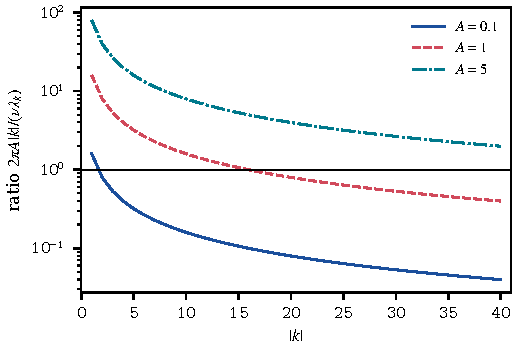
\includegraphics[width=0.75\textwidth]{mf_tg}
\caption{Ratio of advective coupling to viscous decay, $2\pi A|k|/(\nu\lambda_k)$ with $\lambda_k=4\pi^2|k|^2$ (the unit torus), for the linearized Navier Stokes equation about the Taylor Green vortex of amplitude $A$, $\nu=0.01$; the horizontal line marks one. Where the ratio exceeds one the nonlinear correction $\Kcal$ to the Stokes information operator matters; where it is small the Stokes formulas of Section~\ref{m:sec:heat} govern the posterior. The crossover scale grows linearly in $A/\nu$.}\label{m:fig:tg}
\end{figure}

\subsection{The sufficient statistic and the pipeline}

Definition~\ref{m:def:summary} specializes as follows. Given a preliminary estimate $\bar\theta_N$ from one half of the data (for Taylor Green, a few mode least squares fit of its early observations), compute, on the observations of the other half:
\begin{enumerate}[nosep]
\item the nonlinear forward solve $u_{\bar\theta_N}$ on $[0,T]$ by a pseudospectral method, and the residuals $r_i=Y_i-u_{\bar\theta_N}(t_i,x_i)$;
\item the adjoint linearized solve: $w$ solves, backward in time,
\[
\begin{split}
-\partial_sw+\nu Aw+{}&B[u_{\bar\theta_N},\cdot]^*w+B[\cdot,u_{\bar\theta_N}]^*w\\
&=\sum_ir_i\,\delta_{x_i}\delta_{t_i},\qquad w(T)=0,
\end{split}
\]
where the adjoints of the advection terms are, by Proposition~3.1(i) of Konen and Nickl~\cite{konennickl2026} and a direct computation, $B[u,\cdot]^*w=-B[u,w]$, which uses $\nabla\cdot u=0$ and periodicity, and $B[\cdot,u]^*w=P[(\nabla u)^\top w]$, in which $\nabla u$ is the Jacobian $(\nabla u)_{ij}=\partial_ju_i$, so that $\big((\nabla u)^\top w\big)_j=\sum_i w_i\partial_ju_i$; then $\I^*_{\bar\theta_N}r=w(0)$;
\item the application of $(F_N+\Sigma_0^{-1})^{-1}$, with $F_N$ the realized information of Remark~\ref{m:rem:reg}, by conjugate gradients (CG) preconditioned with the explicit Stokes inverse $2\nu(-\Delta)(\Id-S_{2T})^{-1}$ from \eqref{m:eq:fredholm}, each iteration costing one tangent solve and one adjoint solve.
\end{enumerate}
The output is \eqref{m:eq:regsummary}, the summary we compute (Remark~\ref{m:rem:reg}); with $(\I^*_{\bar\theta_N}\I_{\bar\theta_N})^{-1}$ in step 3 and $p_N$ applied to $w(0)$ before it, it is \eqref{m:eq:onestep} for one fold, and its average over the two folds, projected onto the first $J_N$ Stokes modes, is the summary $\hat S_N$ of Definition~\ref{m:def:summary}. Steps 1 and 2 are one gradient evaluation of 4DVar, and step 3 is a Gauss Newton solve. The GBC generator then learns the map from the summary to posterior draws, which by Remark~\ref{m:rem:affine} is asymptotically the identity plus the scale $T(\I^*\I)^{-1}/N$, whose diagonal is the Stokes scale of Table~\ref{m:tab:iota} corrected by the Taylor Green coupling at low $|k|$.

\subsubsection{What Konen Nickl's theorem says for this example} With $\alpha>12$, $\theta_0=u_{\rm TG}(0)$ smooth, and $T_0=0$: the posterior on $\theta$ is asymptotically $N(\tilde\theta_N,T(\I^*_{\theta_0}\I_{\theta_0})^{-1}/N)$ in $\Hds{-\sigma}$, $\sigma>9$; the posterior on $u_\theta(t)$ for $t\in[t_{\min},t_{\max}]$ is asymptotically the Gaussian field solving \eqref{m:eq:tangentgen} with initial datum from that law, at rate $1/\sqrt N$ in supremum norm; a credible band of posterior probability $1-\beta$ around $u_{\tilde\theta_N}$ has frequentist coverage $\to1-\beta$; and no estimator does better in local asymptotic minimax sense. The Taylor Green structure lets one see the covariance: it is the Stokes covariance on the diagonal, modified at $|k|\lesssim A/(2\pi\nu)$ on the unit torus (at $|k|\lesssim A/\nu$ on the $2\pi$ torus) by the nearest neighbor coupling, and the modification is a compact operator so it does not change the tightness range or the RKHS. For the advection functional $\Phi_t(u)=(u\cdot\nabla)u$ at time $t$, the delta method of Section~2.4 of Konen and Nickl~\cite{konennickl2026} gives a $\sqrt N$ Gaussian limit for $\Phi_t(u_{\tilde\theta_N})$, and for Taylor Green $\Phi_t(u_{\rm TG})$ is a gradient field, so the limit describes the fluctuation of the pressure gradient.

\subsubsection{The pipeline} The Navier Stokes pipeline is: pseudospectral simulations from a localized proposal (Step 1 of Algorithm~\ref{m:alg:gbc}, as amended in Algorithm~\ref{m:alg:loc}); per simulated data set, the summary \eqref{m:eq:regsummary} computed above; an identity skip quantile network with a learned scale (Step 2); evaluation at the observed summary (Step 3); forward simulation of the draws (Step 4), or by Corollary~\ref{m:cor:commute} simulation of the tangent equation from the Gaussian limit. With observations on $[T_0,T]$, $T_0>0$, Table~\ref{m:tab:iota} says which modes are lost; the pipeline is unchanged, and the scale learned in Step 2 becomes enormous for $|k|\gtrsim(\nu T_0)^{-1/2}$, which is correct.

\subsection{What survives a realistic design}\label{m:sec:designrobust}

The design in \eqref{m:eq:model} is $N$ points drawn independently and uniformly on $[0,T]\times\Omega$. Real observing systems are not that: they are fixed stations, satellite swaths on repeat orbits, radiosondes at synoptic hours, with errors correlated in space and between channels, and with observation operators, radiances or column integrals, that are not point evaluations.

\emph{Design robust.} Everything that holds for an arbitrary set of design points or depends on the design only through its information operator. Let $\varpi$ be any probability measure on $[0,T]\times\Omega$ and define $\langle h,\I^*_\varpi\I_\varpi h\rangle=\int|\I_\theta h|^2\,d\varpi$, which for the uniform design of \eqref{m:eq:model} is $T^{-1}\langle h,\I^*\I h\rangle$. Lemma~\ref{m:lem:adjoint}, Proposition~\ref{m:prop:linsuff}, Lemma~\ref{m:lem:exact} and Theorem~\ref{m:thm:gap} hold verbatim, and so does the first part of Theorem~\ref{m:thm:locbias}, the mean and variance \eqref{m:eq:varR} of the residual. The regularized summary of Remark~\ref{m:rem:reg} uses the realized information of the design actually drawn and needs no change, and Definition~\ref{m:def:summary} holds with $(\I^*_\varpi\I_\varpi)^{-1}$ in place of $T(\I^*\I)^{-1}$, given pilot estimators with the rates it asks for under $\varpi$. Theorem~\ref{m:thm:main} carries over once the Bernstein von Mises theorem and the conditions behind it are assumed to hold under $\varpi$ (Theorem~\ref{m:thm:nickl2} is proved for independent uniform times and points). Proposition~\ref{m:prop:radius} carries over once Conditions 2A to 2D hold with $\varpi$ in place of the uniform measure and the per coordinate form of Theorem~\ref{m:thm:locbias}, on which its term $\beta(c)$ rests, is available; that form needs the information operator to commute with the prior covariance. For the heat and Stokes equations a design that is uniform in space at each time, whatever the law of the times, keeps $\I^*_\varpi\I_\varpi$ diagonal in $(e_j)$, with the per mode information $\int e^{-2\nu\lambda_jt}\,d\varpi$ in place of $\iota_j$; under a design that is not uniform in space $\I^*_\varpi\I_\varpi$ is in general not diagonal. Correlated errors are equally harmless: with noise covariance $\Sigma_\varepsilon$ in place of $\varsigma^2\Id$, replace $\I^*\I$ by $\I^*\Sigma_\varepsilon^{-1}\I$ throughout and the adjoint statistic by $\I^*\Sigma_\varepsilon^{-1}r$, one extra linear solve. Observation operators that are not point evaluations are the same statement: if observation $i$ reports $\langle A_iu,\cdot\rangle$ rather than $u(t_i,x_i)$, the adjoint is driven by $\sum_ir_iA_i^*$ in place of $\sum_ir_i\delta_{X_i}$.

\emph{Not design robust.} Three things use the i.i.d. uniform design itself. Proposition~\ref{m:prop:gram} is a matrix Bernstein bound and needs independent summands, as do the second moment bounds on the whitened Gram matrix behind Propositions~\ref{m:prop:regheat} and~\ref{m:prop:regfixed}; under a correlated or deterministic design each must be replaced by a bound for dependent or fixed designs, and the concentration of $\Phi^\top\Phi$ on $N\,\diag(\iota_j)$ that Remark~\ref{m:rem:reg} warns about is exactly what degrades. The closed forms $\iota_j=\tfrac1T\int_0^Te^{-2\nu\lambda_jt}dt$ of \eqref{m:eq:iota} and the numbers in Table~\ref{m:tab:iota} are the uniform design values and change under any other $\varpi$; a fixed station network, for instance, samples $\Omega$ on a lattice and aliases modes above its Nyquist frequency, which no amount of data repairs. And the identification of $J_N$ with $N\delta_N^2$ presumes the law of large numbers (LLN) limit of the uniform design; under a design that never visits part of $\Omega$, the relevant dimension is set by the reachable subspace instead.

The practical reading is that the method transfers and the numbers do not. An implementer should recompute $\I^*_\varpi\I_\varpi$ for the observing system at hand rather than reuse $\iota_j$, and should expect Remark~\ref{m:rem:reg}'s regularized summary to matter more, not less, since a realistic design is further from its LLN limit than a uniform one. Every experiment reported in Section~\ref{m:sec:experiments}, the Navier Stokes run included, uses the uniform design of \eqref{m:eq:model}.

\section{Experiments}\label{m:sec:experiments}

Everything reported here is produced from fixed seeds by scripts that are supplied, with their recorded outputs, as ancillary files of our paper~\cite{polsonsokolov2026manifold} and described in Appendix~\ref{app:code}. The generator \texttt{make\_experiments\_tex.py} wrote the experiments section of that paper, tables included, directly from the resulting \texttt{json}, so every measured number in the tables and in the figure comes from a recorded run rather than being transcribed by hand. The setting is the heat equation of Section~\ref{m:sec:heat} on $\Omega=[0,1]$ with $\nu=0.01$, $T=1$, the fixed prior of that section with $\alpha=3$, and the conjugate Gaussian posterior available in closed form, so that the exact posterior is known and every approximation can be measured against it rather than against another approximation.

\subsection{The finite $N$ check, in the regime where the data speak}\label{m:sec:expfinite}

Table~\ref{m:tab:diag} reports the diagnosis. The first row is the uncalibrated setting of panel (a) of Figure~\ref{m:fig:heatgbc}, $\rho=1$ and $N=2000$: no mode has data precision exceeding prior precision. The agreement with the Bernstein von Mises scale there, $1.43\times10^{-4}$, is therefore not a validation of anything: both sides of the comparison are the prior, and a diagnostic that compares the prior with itself is vacuous whatever number it returns.

Two things are wrong at once and they have to be separated. The first is the scale of the prior, which $\rho$ fixes: calibrating $\rho$ so that the prior standard deviation at $|k|=1$ matches the initial condition there gives $\rho=124.0$, moves $k_{\rm eff}$ from $0$ to 2, covers every informed mode, and brings the relative $L^2$ error to $0.257$. The second is the shape: the initial condition $\theta_{0,k}=(1+k^2)^{-1}\mathrm{sign}(\sin k)$ decays like $k^{-2}$ whereas a draw from the fixed prior with $\alpha=3$ decays like $k^{-3}$, so after calibration the worst mode is still $39.9$ prior standard deviations out. That tail is invisible while $k_{\rm eff}$ is small and becomes visible as $N$ grows: the informed modes covered go from 2 of 2 at $N=2\times10^3$ to 3 of 5 at $N=1.3\times10^6$, with the worst standardized error over informed modes rising to $7.91$. Nothing is wrong with the posterior; the prior is wrong about the truth, and more data is what reveals it.

The last three rows replace the fixed $\theta_0$ by a draw from the prior itself, the only setting in which nominal coverage is the right thing to expect. Relative $L^2$ error stays near one at the smaller two, which is not a failure: this draw is small, with norm $0.0208$ against a prior root mean square norm of $0.50$, and the posterior standard deviations of its informed modes are of the same size ($0.027$ and $0.034$ at $N=2\times10^3$), so the error of the posterior mean is of the size of the signal itself and a ratio above one can occur while every informed mode stays within $2.2$ posterior standard deviations. Section~\ref{m:sec:resolution} says how many modes the data can resolve.

\begin{table}[t]\centering\footnotesize\setlength{\tabcolsep}{3pt}
\caption{The finite $N$ check for the heat equation. $k_{\rm eff}$ is the number of modes with $N\iota_k\ge\rho^{-2}\lambda_k^\alpha$; ``truth/prior sd'' is $\max_k|\theta_{0,k}|/\sigma_{0,k}$, a measure of how atypical the truth is under the prior; the coverage columns count the modes whose truth lies within two posterior standard deviations, over the informed modes and over all twenty; with $k_{\rm eff}$ this small these are counts and not estimates of a coverage probability, for which see the replicate study of Section~\ref{m:sec:expstudy}; $|z|_{\max}$ is the largest standardized error over informed modes; and the last column is the largest relative discrepancy, over all twenty modes, between the exact posterior standard deviation and the Bernstein von Mises (BvM) scale with the prior precision added, $(N\iota_k+\sigma_{0,k}^{-2})^{-1/2}$. The truth of the last block is a fixed draw from the prior that is typical in each coordinate but small in norm.}\label{m:tab:diag}
\begin{tabular}{rrrrrrrrr}
\toprule
$N$ & $\rho$ & $k_{\rm eff}$ & \shortstack[r]{truth/\\prior sd} & \shortstack[r]{cov.\\inf.} & \shortstack[r]{cov.\\all} & $|z|_{\max}$ & \shortstack[r]{rel.\\$L^2$} & \shortstack[r]{BvM\\rel.}\\
\midrule
\multicolumn{9}{@{}l}{Uncalibrated prior}\\
$2\times10^3$ & 1 & 0 & 4948.6 & n/a & 0 of 20 & n/a & 0.982 & $1.43\times10^{-4}$ \\
\addlinespace
\multicolumn{9}{@{}l}{Calibrated $\rho$}\\
$2\times10^3$ & 124 & 2 & 39.9 & 2 of 2 & 2 of 20 & 1.96 & 0.257 & $6.05\times10^{-3}$ \\
$5\times10^4$ & 124 & 3 & 39.9 & 3 of 3 & 3 of 20 & 0.92 & 0.144 & $1.60\times10^{-3}$ \\
$1.3\times10^6$ & 124 & 5 & 39.9 & 3 of 5 & 3 of 20 & 7.91 & 0.081 & $7.77\times10^{-4}$ \\
\addlinespace
\multicolumn{9}{@{}l}{Fixed draw from the prior}\\
$2\times10^3$ & 124 & 2 & 1.9 & 2 of 2 & 20 of 20 & 0.59 & 1.007 & $6.05\times10^{-3}$ \\
$5\times10^4$ & 124 & 3 & 1.9 & 2 of 3 & 19 of 20 & 2.18 & 1.270 & $1.60\times10^{-3}$ \\
$1.3\times10^6$ & 124 & 5 & 1.9 & 5 of 5 & 20 of 20 & 1.54 & 0.250 & $7.77\times10^{-4}$ \\
\bottomrule
\end{tabular}
\end{table}

\subsection{Cost and accuracy against the alternatives}\label{m:sec:expcost}

Table~\ref{m:tab:cost} reports what one analysis costs. Unless a variant is named, GBC in this table and in the rest of this section is Algorithm~\ref{m:alg:loc} with $c=2$ and the identity head, applied to the regularized summary of Remark~\ref{m:rem:reg}. The units are forward or adjoint solves of the linearized equation, which is the currency in which data assimilation is priced, together with wall clock for the methods actually run here. The two comparators are the Laplace approximation at the posterior mode and the preconditioned Crank Nicolson sampler (pCN), in the form given by Cotter and coauthors~\cite{cotter2013}.

\begin{table}[t]\centering\footnotesize\setlength{\tabcolsep}{4pt}
\caption{Cost and accuracy for one analysis of the heat equation, $N=50000$, $|k|\le8$, single core. Errors are the maximum over the retained modes, in units of the exact posterior standard deviation (psd). ``Amortized'' records whether a second data set can be analyzed without repeating the cost. $\dagger$: analytic, not measured. In this linear Gaussian model both the Laplace approximation at the posterior mode and the GBC generator have the exact posterior mean, by Proposition~\ref{m:prop:linsuff}, so their mean error is exactly zero at every budget. The standard deviation ratio, the median over the retained modes of the reported posterior standard deviation divided by the exact one, is the column that carries information here. Neither the $8000$ solves of GBC, a forward and an adjoint solve for each of its $M=4000$ simulations, nor the $2$ of Laplace, one forward and one adjoint solve, include forming the Gauss Newton covariance $(\Phi^\top\Phi+\Sigma_0^{-1})^{-1}$, which is the covariance of the Laplace row and which GBC's localized proposal and summary also use. It is formed once in either method and takes one further linearized solve per retained mode, $8$ here; the Laplace time is that of forming it from $\Phi$, and the GBC time, which covers the simulations, the fit and the $4000$ draws, leaves it out.}\label{m:tab:cost}
\begin{tabular}{lrrrrl}
\toprule
Method & Solves & Time (s) & \shortstack[r]{Max err.\\(psd)} & \shortstack[r]{sd\\ratio} & Amortized\\
\midrule
GBC, Algorithm~\ref{m:alg:loc}, $c=2$ & 8000 & 2.91 & $0^{\dagger}$ & 1.003 & amortized \\
Laplace at $\hat S_N$ & 2 & 0.0003 & $0^{\dagger}$ & $1^{\dagger}$ & no \\
pCN, $2\times10^{5}$ iterations & 200000 & 86.5 & 0.325 & 0.947 & no \\
\bottomrule
\end{tabular}
\end{table}

Three readings. First, GBC is not more accurate than Laplace and cannot be: by Definition~\ref{m:def:gen} its generator is a Monte Carlo estimate of the Laplace approximation, so its mean is that approximation's mean exactly, and the $0.016$ posterior standard deviations one reads off the worst of its $4000$ output draws is the sampling error of those draws, not an error of the method. What it buys over Laplace is that the forward map is reached only by simulation and that no Hessian is evaluated at the training draws: the one Gauss Newton covariance of Algorithm~\ref{m:alg:loc} is formed once, at the preliminary estimate (Remark~\ref{m:rem:whichcov}). Second, pCN is included to exhibit the Monte Carlo rate the two methods share, not as a tuned competitor: in this conjugate model the exact posterior is a known Gaussian that can be sampled directly and a whitened or Gibbs sampler would mix in one step, so the comparison is not in GBC's favor on a single data set: $200000$ iterations and a tuned acceptance rate of 0.246 at $\beta=0.0491$ deliver a minimum effective sample size of 16 across the retained modes, which is why its worst mode error is larger than GBC's and is Monte Carlo noise rather than bias: its posterior standard deviation ratio is 0.947. Given enough iterations pCN is exact and GBC is not. Third, the cost that matters operationally is the ratio to a 4DVar minimization. Neither 4DVar nor an ensemble Kalman filter (EnKF) is run here: a 4DVar minimization returns a point estimate, and an ensemble filter returns an ensemble that is a posterior sample only for a linear forward map and a large ensemble, so no error in these units is reported for either. Both do have conventional solve counts: 20 for a Gauss Newton 4DVar at ten inner iterations of one forward and one adjoint solve, and one solve per ensemble member for an ensemble filter. Against those conventions one GBC analysis is 400 4DVar equivalents at $M=4000$ and 80 times a 100 member EnKF. Those are the numbers Section~\ref{m:sec:related} refers to, and they are the price of amortization: the 4000 simulations are spent once, and every subsequent data set is a forward pass.

\subsection{Error against cost, and coverage over replicates}\label{m:sec:expstudy}

The error against cost and the coverage over replicates are both studied at $N=50000$ with $D=8$ modes retained, of which $k_{\rm eff}=3$ are data dominated, and at the calibrated $\rho=124$ of Section~\ref{m:sec:expfinite}. A single realization cannot separate a miscalibrated posterior from an unlucky draw, so calibration is checked over replicates, on three truth arms. The result, set out in Section~\ref{m:sec:covstudy} and shown for the arm drawn from the prior in the lower panel of Figure~\ref{m:fig:cost}, is that GBC reproduces whatever the exact posterior does, on every arm, under a paired McNemar test that takes the replicate as its unit.

In the linear Gaussian model of Section~\ref{m:sec:heat} Proposition~\ref{m:prop:linsuff} gives the mean map in closed form, so GBC's posterior mean is exact at every budget and only the $D\times D$ covariance is estimated from the $M$ simulations. Scoring the mean therefore measures nothing about the method: over 40 replicates and 8 budgets, 320 measurements in all, its error is exactly zero (Remark~\ref{m:rem:artifact}).

\begin{remark}[Why a finite draw mean error is not an approximation floor]\label{m:rem:artifact}
Scoring GBC's posterior mean against the exact one in this model measures a quantity whose value is exactly zero, so any nonzero reading is the sampling noise of however many output draws were taken. Holding that count fixed at 4000 while the simulation budget sweeps a factor of 128 returns 0.023 to 0.044 posterior standard deviations with a fitted slope against the budget of $-0.029$, flat. That flatness is not an approximation floor of the plug in generator. The quantity decays in the number of output draws, not in $M$, so no simulation budget can move it and there is nothing there to converge. A Gaussian head does carry a genuine approximation error wherever the posterior is not Gaussian, but a linear Gaussian benchmark is precisely the case in which that error vanishes identically, so this diagnostic cannot measure it at any budget. Any study of a Gaussian head generator that scores the mean on a conjugate benchmark meets the same trap.
\end{remark}

What the simulations buy is the covariance, and scored analytically it converges at the Monte Carlo rate with no floor. Across the 3 generator variants and both covariance metrics the fitted slope of $\log$ error against $\log$ solves lies between $-0.521$ and $-0.495$ against a nominal $-1/2$, with replicate standard error 0.009; raising $M$ from 250 to 32000 cuts the error on the standard deviations from 0.081 to 0.0071. The learned mean variant, which ignores Proposition~\ref{m:prop:linsuff} and regresses $\theta$ on the summary from the same simulations, does carry a mean error, converging at $-0.514$ to 0.030 at the largest budget: that gap is what the affine structure is worth. pCN has no floor either. Its error on the standard deviations falls from 0.577 to 0.053 as the budget grows from $5.0\times10^{3}$ to $1.3\times10^{6}$ solves. Its rate has to be read with the mixing in view: the minimum effective sample size over the retained modes is 4 at the smallest budget and 131 only at the largest, so the smallest budgets measure how far the chain has failed to move rather than a Monte Carlo error. Fitting all 5 gives $-0.423$; fitting the 3 budgets with an effective sample size above 7 gives $-0.507$, which is the Monte Carlo rate and is what we use below.

So both methods converge at essentially the same rate, $-0.521$ for GBC against $-0.507$ for pCN on the standard deviations. The advantage is therefore a constant factor rather than a widening gap, and it can be read off without extrapolating either curve beyond where it was measured. Over the band of accuracy both methods reached, 0.081 down to 0.053 posterior standard deviations, pCN needs between 1154 and 1181 times as many solves as GBC to match it on the standard deviations, and between 366 and 510 times as many on the full covariance, over the band 0.140 down to 0.063 of relative error in Frobenius norm that both reached on that metric. Solves, not seconds, are the currency: wall clocks depend on the machine and its load (Appendix~\ref{app:code} records a rerun on a busier machine). The choice between the two methods turns on how many solves an application can afford.

\begin{figure}[tp]\centering
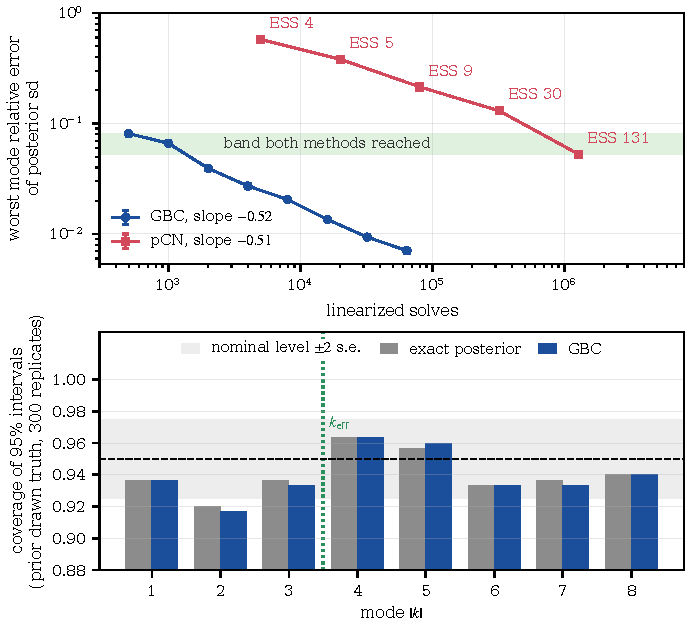
\includegraphics[width=0.94\textwidth]{mf_cost}
\caption{Upper panel: error against the number of linearized solves, on the metric the simulations actually control. GBC's posterior mean is exact at every budget in this model (Proposition~\ref{m:prop:linsuff}), so what is plotted is the error of the estimated posterior standard deviations, in units of the exact ones, taken as the largest over the retained modes and averaged over 40 replicates, for GBC at $M=250$ to $32000$ and for pCN at $5.0\times10^{3}$ to $1.3\times10^{6}$ iterations; the bars are one standard error over replicates, and the labels give the minimum over modes of the effective sample size (ESS) of the pCN chain, averaged over replicates. Both follow the Monte Carlo rate and neither has a floor. The shaded band is the range of accuracy both reached. Lower panel: coverage of nominal $95\%$ credible intervals by mode, over 300 replicates of the arm in which $\theta_0$ is drawn from the prior, for the exact posterior and for GBC; the shaded band is the nominal level plus or minus two binomial standard errors, and the dotted line marks $k_{\rm eff}$, beyond which the intervals are the prior's. Over the 2400 (replicate, mode) pairs of that arm the two disagree on 5 pairs against 3, each in a different replicate, a coverage difference of 0.0008 (Table~\ref{m:tab:cover}).}\label{m:fig:cost}
\end{figure}

\subsection{Coverage over replicates, in full}\label{m:sec:covstudy}

Table~\ref{m:tab:cover} has the numbers in full. Hypothesis (G1) of Assumption~\ref{m:ass:G} is stated in $P^\N_{\theta_0}$ probability at a \emph{fixed} $\theta_0$, and redrawing $\theta_0$ from the prior at every replicate makes the exact posterior's coverage nominal by construction, so under that design alone the comparison cannot fail informatively. The three arms are therefore $\theta_0$ redrawn from the prior, a fixed typical draw, and a fixed rough truth $\theta_{0,k}=(1+k^2)^{-1}\mathrm{sign}(\sin k)$, which the prior charges only in its tail. With $M=4000$ simulations, each arm has 300 replicates.

\begin{table}[t]\centering\footnotesize\setlength{\tabcolsep}{4pt}
\caption{Coverage of nominal $95\%$ credible intervals over 300 replicates per arm, by truth arm. ``All'' is over the $D=8$ retained modes, ``informed'' over the $k_{\rm eff}=3$ modes in which data precision exceeds prior precision. $b/c$ are the discordant counts, the (replicate, mode) pairs that the exact posterior covers and GBC misses and the reverse, out of $2400$. With $x_r$ the number of modes of replicate $r$ that the exact posterior covers and GBC misses minus the number of the reverse, $z=\sum_rx_r/(\sum_rx_r^2)^{1/2}$ is the clustered McNemar statistic of Durkalski and coauthors~\cite{durkalski2003}, and $p$ is the exact two sided $p$ value of the sign flip test, which gives each nonzero $x_r$ an independent random sign, as it has when the two methods are exchangeable within a replicate. The rough arm is misspecified by construction: its truth decays like $k^{-2}$, whereas a draw from the prior of smoothness $\alpha=3$ used here decays like $k^{-3}$, so both methods undercover, and identically; a draw from a prior with $\alpha>12$, the smoothness that Konen and Nickl~\cite{konennickl2026} require for the Navier Stokes problem, decays faster still. That the exact posterior undercovers too is the point of including the arm.}\label{m:tab:cover}
\begin{tabular}{>{\raggedright\arraybackslash}p{1.5in}ccccccc}
\toprule
& \multicolumn{2}{c}{All modes} & \multicolumn{2}{c}{Informed modes} & & & \\
\cmidrule(lr){2-3}\cmidrule(lr){4-5}
Truth arm & exact & GBC & exact & GBC & $b/c$ & $z$ & $p$\\
\midrule
$\theta_0\sim\Pi$, redrawn each replicate & 0.940 & 0.940 & 0.931 & 0.929 & $5$/$3$ & $0.71$ & $0.73$\\
fixed typical draw & 0.843 & 0.845 & 0.914 & 0.919 & $2$/$6$ & $-1.63$ & $0.22$\\
fixed rough truth & 0.251 & 0.251 & 0.670 & 0.670 & $1$/$1$ & $0.00$ & $1.00$\\
\bottomrule
\end{tabular}
\end{table}

Two things separate here. First, the exact posterior does not have frequentist coverage at a fixed truth and is not required to: its coverage over all $D$ retained modes falls from 0.940 on the prior drawn arm to 0.843 at the fixed typical draw and 0.251 at the rough one. That is the shrinkage of the posterior mean, milder on the informed modes, which averaging over the prior hides; as $N\to\infty$ each mode is covered at the nominal rate, with $D=8$ as here and, by Proposition~\ref{m:prop:regfixed}, with $D$ growing, but slowly at the rough truth.

Second, and this is the claim we make, GBC reproduces whatever the exact posterior does. Both methods are scored on the same replicate and the same mode, so the yardstick is a paired comparison, McNemar's, and not the binomial standard error of a single coverage estimate. The pairs of one replicate are not independent, since its eight modes are computed from the same data, so the comparison is made over the 300 independent replicates: the statistic of Table~\ref{m:tab:cover} is $z=\sum_rx_r/(\sum_rx_r^2)^{1/2}$. Where no replicate holds more than one discordant pair, as on the prior drawn and the rough arm, that statistic and its exact test are McNemar's own; on the typical arm one replicate holds one discordant pair of each kind. The standard error that the test gives the difference of the coverages, $(\sum_rx_r^2)^{1/2}/2400$, is between 11 and 21 times smaller than the binomial standard error at the nominal level of the coverage of a single mode over the 300 replicates, and between 5 and 7 times smaller than the standard error of the difference of the coverages over all modes of two methods run on independent data, so the test is several times more sensitive than the comparison it replaces. GBC survives it on every arm. The largest discrepancy across the three is 1.63 standard errors, on the typical arm, with exact $p$ value 0.22, and the largest difference in coverage over all modes is 0.0017; on the rough arm, where the exact posterior covers barely a quarter of the time, the two disagree on $2$ of $2400$ pairs, one each way.

The calibration claim is therefore relative rather than absolute: GBC reproduces the posterior it targets, including where that posterior is badly miscalibrated as a frequentist procedure. Coverage at a fixed truth is a property of the prior and the model rather than of the computation. One qualification: both arms of the comparison use the same summary, the adjoint statistic of Lemma~\ref{m:lem:adjoint}, and, by Proposition~\ref{m:prop:linsuff}, the same closed form posterior mean, so what differs between them is the covariance, exact in one case and estimated from the $M$ simulations in the other. The agreement is evidence that the estimated covariance is right, and is not a test of the summary or of the centering.

\subsection{A nonlinear check: two dimensional Navier Stokes}\label{m:sec:expns}

The experiments above are conjugate by design. This one is not, and it is the test that matters for Sections~\ref{m:sec:loc} and~\ref{m:sec:ns}: whether the localization theory survives contact with a nonlinear forward map. We solve \eqref{m:eq:nsproj} in vorticity form on the $2\pi$ periodic torus by a pseudospectral method with two thirds dealiasing and Heun stepping, on a $24^2$ grid with $\nu=5\times10^{-3}$, $T=1$ and $80$ steps; one forward solve costs about $15$\,ms. The unknown is the initial vorticity in $D=6$ real cosine modes with wavevectors $(1,0),(0,1),(1,1),(1,-1),(2,0),(0,2)$, the prior is independent Gaussian with standard deviations $1.5(\lambda_j/\lambda_1)^{-1}$, and the truth is a prior draw. The data are $N=80$ space time points with both velocity components observed, noise $\sigma=0.45$ against a signal of standard deviation about $0.95$, and observation times uniform on $[0,T]$, so the theory applies in its $T_0=0$ form. Accuracy is the per coordinate $\Wone_1$ distance to an adaptive random walk Metropolis reference, computed as the mean absolute difference of the two quantile functions at $199$ equally spaced levels from $0.005$ to $0.995$, normalized by that coordinate's posterior standard deviation and averaged over coordinates. The reference chain runs $6000$ iterations and keeps the last $4500$, with a Gaussian proposal of the Laplace covariance whose scale is adapted every $200$ iterations toward an acceptance rate of $0.30$; its effective sample size is about $250$ per coordinate. The generators of this section use the summary \eqref{m:eq:regsummary} at the maximum a posteriori estimate, with its Jacobian by finite differences (two Gauss Newton steps in the lower panel of Table~\ref{m:tab:ns}), and resample their training residuals rather than draw the Gaussian noise of Definition~\ref{m:def:gen}. The comparator is the Laplace approximation at the maximum a posteriori estimate, which in this six mode truncation is the finite sample form of the classical parametric Bernstein von Mises limit, the finite dimensional counterpart of the limit of Konen and Nickl~\cite{konennickl2026}, and is free: one Gauss Newton solve and one Hessian.

\begin{table}[tp]\centering\footnotesize
\caption{Two dimensional Navier Stokes, $D=6$, $N=80$. Distance to the Metropolis reference in units of posterior standard deviation, per coordinate and averaged; lower is better. The upper panel varies the architecture at $M=1600$, with a one step summary and, in the localized rows, radius $c=3$; the lower panel applies the three corrections of Section~\ref{m:sec:loc} in turn, at $c=5$, $M=1100$ and $k=2$ Gauss Newton steps (Remark~\ref{m:rem:nsdiag}). Every script scores against the same reference chain and draws its own Laplace sample, so the Laplace row moves between panels; across the six runs it lies between $0.076$ and $0.083$. The last row of that panel adds to the rescaled generator a shift of the center by the cubic correction of Remark~\ref{m:rem:relin}, the third derivative term of the Laplace expansion of the posterior mean, which is not a step of Algorithm~\ref{m:alg:loc}; on the same draws that shift raises the error of the rescaled generator from $0.070$ to $0.072$, that of the centered generator from $0.091$ to $0.092$ and that of the Laplace approximation from $0.078$ to $0.081$. Over twenty further resamplings of the $8000$ draws of the rescaled generator the shift raises its error in every one of them, by $0.002$ to $0.003$. The last line is not a method: it is the Monte Carlo standard error of the reference's own posterior mean.}\label{m:tab:ns}
\begin{tabular}{@{}>{\raggedright\arraybackslash}p{3.3in}c@{}}
\toprule
& \shortstack{$\Wone_1$ /\\ posterior s.d.}\\
\midrule
\multicolumn{2}{@{}l}{\emph{Architecture, $M=1600$}}\\
\quad training from the prior, identity head & 1.077\\
\quad training from the prior, learned affine head & 0.901\\
\quad training from the prior, $K=200$ nearest summaries, affine head & 0.364\\
\quad localized training, identity head & 0.187\\
\quad localized training, learned affine head & 0.180\\
\midrule
\multicolumn{2}{@{}l}{\emph{The corrections of Section~\ref{m:sec:loc}, $c=5$, $k=2$, $M=1100$}}\\
\quad localized, uncentered, spread as measured & 0.136\\
\quad $+$ residuals centered, Theorem~\ref{m:thm:locbias}(ii) & 0.092\\
\quad $+$ spread rescaled, Theorem~\ref{m:thm:locbias}(iii) & 0.070\\
\quad $+$ center shifted by the cubic correction, Remark~\ref{m:rem:relin} & 0.072\\
\midrule
Laplace at the maximum a posteriori estimate & 0.078\\
\midrule
\emph{Monte Carlo error of the reference itself} & \emph{0.063}\\
\bottomrule
\end{tabular}
\end{table}

Table~\ref{m:tab:ns} reads as a sequence of corrections, each one predicted by Section~\ref{m:sec:loc}.

\emph{Prior training with the identity head fails, and does not improve with $M$.} The error is about one posterior standard deviation and moves from 1.131 at $M=400$ to 1.078 at $M=800$ and 1.077 at $M=1600$, so it is bias and not Monte Carlo error. This is the shrinking neighborhood caveat of Remark~\ref{m:rem:affine} made concrete: the identity head is justified on the localization set, draws from the prior lie far outside it, and there the summary \eqref{m:eq:regsummary}, whose Jacobian sits at the preliminary estimate, is not a one step efficient estimator but an arbitrary linear functional. Learning an affine head instead recovers only part of the loss, because the map is genuinely nonlinear over the prior's support.

\emph{Localization is necessary, and post hoc localization is not a substitute.} Drawing the training parameters from a proposal centered at the preliminary estimate cuts the error by a factor of 5.8 and restores the decrease in $M$. Localizing a prior trained pool after the fact by keeping the $K$ nearest summaries reaches only 0.364 at $K=200$ and degrades as $K$ grows, which is the bias variance trade off of approximate Bayesian computation and is why Algorithm~\ref{m:alg:loc} localizes the proposal rather than the pool.

Two further knobs, importance weighting the localized draws back to the prior and relinearizing the summary, are reported in Remark~\ref{m:rem:nsdiag}.

\emph{The residual mean is the one Theorem~\ref{m:thm:locbias}(ii) predicts.} The uncentered head, which resamples the training residuals, adds their sample mean to the observed summary, and so displaces its center. Per coordinate that mean is right in sign and within $0.09$ posterior standard deviations in magnitude of the linear Gaussian prediction $P\bar\theta_N$ of Theorem~\ref{m:thm:locbias}(ii), the measured mean being the smaller in five of the six coordinates (both vectors are in Section~\ref{m:sec:loc}). We attribute the difference to the nonlinearity of the map; this run does not isolate it, since the sampling error of a mean of $M=1100$ residuals is about $0.03$ posterior standard deviations and four of the six differences are no larger than that. Centering removes it, at which point the center of the GBC posterior is displaced from the reference's own posterior mean by 0.061, which is exactly the maximum a posteriori estimate's displacement. Rescaling the spread by the reciprocal of the predicted inflation $(s_j+c^2p_j^2)^{1/2}$ of Theorem~\ref{m:thm:locbias}(iii) brings the error to 0.070, which is where Algorithm~\ref{m:alg:loc} stops; shifting the center as well, by the cubic correction described in the caption of Table~\ref{m:tab:ns}, gives 0.072, so that correction does not help here. In the last coordinate at $c=5$ the theorem predicts an inflation of 1.25, and the standard deviation of the residuals is measured at 1.25 times the Laplace standard deviation, which is 1.18 times the reference's.

Two further regimes were run, each with its own reference chain of $3000$ retained draws, to look for the crossover at which non Gaussianity of the posterior would favor a simulation based method. Both used $N=25$ space time points on $100$ time steps, $M=1200$ draws from a proposal of radius $c=2$, a one step summary and the identity head. The first raises the amplitude, the constant $1.5$ in the prior standard deviations raised to $2$, which raises the proxy $\max_j|\theta_{0,j}|/\nu$ of the advection to dissipation ratio of the realized truth from $185$ at the baseline constants to $246$, still below the $347$ of the main run's truth; the second widens the posterior, with noise standard deviation $1.30$ in place of $0.45$ and that constant raised to $3$ (proxy $370$). With the residuals neither centered nor rescaled, as in the runs recorded with our paper, GBC scored 0.105 and 0.253 against the Laplace approximation's 0.074 and 0.111. With the corrections of Section~\ref{m:sec:loc} applied to the same residuals, centering and then rescaling the spread, GBC scores 0.086 and then 0.080 in the first regime and 0.172 and then 0.114 in the second, so that the corrected generator ends 0.006 and 0.003 above the Laplace approximation, while the resampling noise of a single score is 0.003 to 0.004 for each method and the Monte Carlo standard errors of the two references are 0.081 and 0.083. The crossover was not found, and neither regime made the posterior measurably less Gaussian than the main run. Their mean absolute marginal skewness, 0.10 and 0.13, varies between chain seeds about as much as between regimes (from 0.06 to 0.10 in the first, from 0.07 to 0.13 in the second and from 0.09 to 0.12 at the baseline constants), and it is of the size that sampling error alone gives a Gaussian chain of that length and autocorrelation, 0.09 on average, with 0.05 to 0.15 between the 5th and 95th percentiles; the reference chain of the main run has 0.17, against 0.07 for a Gaussian chain like it. The uncorrected generator lost more in these regimes, where the prior fractions are larger, up to 0.36 and 0.65 against 0.17 in the main run: the displacement and inflation that the two corrections remove grow with the prior fraction (Theorem~\ref{m:thm:locbias}), and once they are removed, what separates GBC from the Laplace approximation is within the noise of the comparison. Both errors are governed by the curvature of $\Gcal$ measured in posterior standard deviations, so they do not move independently and the crossover cannot be assumed.

What the table does not show is a win. Corrected, GBC reaches 0.070 against the Laplace approximation's 0.078, but over resamplings of its own draws its error averages 0.077 with standard deviation 0.005, and the reference's own Monte Carlo standard error is 0.063, so the two are indistinguishable at the resolution available: bringing that standard error down to the size of the difference in the table would need a chain about sixty times longer. In this regime the Laplace approximation is excellent and free, and recommending a simulation based method on accuracy grounds would be wrong. What the table does show is that the distance between a naive GBC implementation and a correct one is a factor of 15 (1.077 at $M=1600$ against 0.070 at $M=1100$), and that every step of that factor is prescribed by Section~\ref{m:sec:loc} rather than being a tuning choice; the cubic correction of the last row is not one of those steps. The case for GBC here is amortization, and the regimes in which it is the only option are the ones the theory excludes: $T_0>0$, model error, non Gaussian noise.

\begin{remark}[Two diagnostics from the Navier Stokes run]\label{m:rem:nsdiag}
\emph{Importance weighting back to the prior degenerates, as the algorithm says it does.} Correcting the localized proposal by weights $w\propto\pi/q$ raises the error of the learned affine head, with the one step summary and $M=1200$, at every radius at which the algorithm operates: from 0.247 to 0.279 at $c=1$, from 0.175 to 0.387 at $c=2$, from 0.172 to 0.327 at $c=3$ and from 0.269 to 0.717 at $c=5$, with effective sample sizes of 29, 6.5, 15 and 1.5 out of $M$. At $c=8$ the weighted error, 0.377 at an effective sample size of 34, is below the unweighted 0.631; the statement concerns the radii $c\le5$ at which the algorithm operates. The proposal is much narrower than the prior, so the weights grow like $e^{+\norm\theta^2}$ in its tails. The unweighted estimator is biased for the prior based posterior, because the proposal acts as a prior on the training draws; in the linear Gaussian model the bias is of first order in the prior fraction (Theorem~\ref{m:thm:locbias}) and, for the affine head, in $c^{-2}$ as well, so it is small when the data dominate the prior and the radius is not small, while the weighted estimator's variance is not.

\emph{Linearizing the summary once is what the $c^4$ term of Proposition~\ref{m:prop:radius} costs.} At $c=2$ and $M=500$ the one step and two step Gauss Newton summaries are indistinguishable for the learned affine head, 0.169 against 0.171, as they must be where the $c^4$ term is negligible. At $c=6$ the one step summary costs that head a factor of 2.3, 0.370 against 0.162, and relinearizing recovers all of it (Remark~\ref{m:rem:relin} gives the iteration and its cost).
\end{remark}

\subsection{What these experiments do not establish}\label{m:sec:expnot}

Most of them are run on a linear, one dimensional, conjugate problem. Those test the summary, the generator and the resolution accounting of Sections~\ref{m:sec:suff}, \ref{m:sec:qnn} and \ref{m:sec:resolution}, and they cannot test the nonlinear theory at all. Section~\ref{m:sec:expns} supplies the nonlinear test. It is a six dimensional Galerkin truncation, which is a small problem; the comparison is against a Metropolis reference whose own Monte Carlo error is of the same size as the differences being reported; and the truth is a prior draw, so nothing there speaks to misspecification. What it does establish is that the three corrections of Section~\ref{m:sec:loc} are the ones that matter on a genuinely nonlinear map, in the direction and roughly the magnitude the theorems predict. Whether the same holds at operational resolution, where $D$ is in the thousands and the reference is unavailable, is left open. Section~\ref{m:sec:ns} remains a specification of the pipeline at the resolution the framework is stated for, not a report of a computation at that resolution.

\section{Nondissipative equations: Schr\"odinger}\label{m:sec:nondiss}

Every theorem so far uses dissipation twice: the parabolic semigroup makes the difference $\I_\theta-\Lcal$ two derivatives smoothing, which is what makes $\Kcal$ compact and allows Fredholm inversion of the information operator; and it makes $\I_{\theta_0}$ continuous from $H^{-k-2}$ into $\Ccal$, which is what lifts the weak topology theorem to the supremum norm.

\subsection{Linear Schr\"odinger}

Let $i\partial_tu=-\Delta u$ on $\T^d$, $u(0)=\theta\in L^2(\T^d;\C)$, so $u_\theta(t)=e^{it\Delta}\theta=\sum_je^{-i\lambda_jt}\theta_je_j$, and observe $Y_i=u_\theta(t_i,x_i)+\varepsilon_i$ with complex Gaussian noise. The forward map is unitary at every time, so the design matrix \eqref{m:eq:design} has $|s_j(t)|=1$ and
\begin{equation}\label{m:eq:schinfo}
\iota_j(T_0)=\frac1{T-T_0}\int_{T_0}^T|e^{-i\lambda_jt}|^2dt=1\qquad\text{for all }j\text{ and all }T_0 .
\end{equation}
\begin{itemize}[nosep]
\item There is no dissipation barrier. The observation window is irrelevant; Table~\ref{m:tab:iota} is replaced by a column of ones. The curvature constant $c_{\min}$ of the localized Langevin algorithm of Nickl and Wang~\cite{nicklwang2024} is $1$ uniformly in $D$ here, and since the forward map is linear and the information is $1$ in every mode, the expected Hessian of the negative log likelihood is $N\,\Id$ at every $\theta$ and gradient stability holds on all of the coefficient space, as for the heat equation in Section~\ref{sec:gradstab}. Their polynomial time guarantee is proved for a related steady state elliptic model, and verifying their remaining conditions for the initial condition of a time evolution equation is open as far as we know (Section~\ref{sec:gradstab}); if the guarantee carries over, the algorithm mixes in time polynomial in $D$ with no exponential factor, and dispersive is computationally easier than dissipative. For the linear equation itself no sampler is needed: the posterior is the Gaussian of Proposition~\ref{m:prop:sch}(a), and one Cholesky factorization of its $D\times D$ precision matrix gives exact draws.
\item The information operator is $T\cdot\Id$ in the unnormalized convention of \eqref{m:eq:modeinfo}; its inverse is bounded on $L^2$, and Condition 2E holds with $L^2$ in place of $H^{-1}$. The Bernstein von Mises limit for the initial condition is $\Ncal_{\theta_0}=N(0,T(\I^*\I)^{-1})=N(0,\Id)$, complex white noise on $\T^d$, tight on $H^{-a}$ for $a>d/2$ rather than $a>1+d/2$. The posterior on $\theta$ is Gaussian with a data independent covariance, so the posterior mean summary is sufficient, exactly and not only asymptotically, and the uniform statement of Assumption~\ref{m:ass:U}, which Theorem~\ref{m:thm:jwbvm} needs in general, is not required here; the sufficient statistic is again the adjoint evolution, with components $(\Phi^*Y)_j=\sum_ie^{i\lambda_jt_i}\overline{e_j(x_i)}Y_i$, i.e.\ the data run backward by the unitary group, and the GBC quantile map is affine, with the per mode scale of Proposition~\ref{m:prop:sch}(a). Statistically, the initial condition is recovered at the nonparametric rate of direct regression: no better than $\delta_N$ in $L^2$, since there is no sense in which the PDE constraint helps.
\item There is no supremum norm trajectory theorem. Since $u_\theta(t)=e^{it\Delta}\theta$ and $e^{it\Delta}$ is an isometry on every $H^s$, the state at time $t$ has exactly the regularity of the initial condition, the posterior standard deviation of $u_\theta(t,x)$ is $N^{-1/2}(\sum_j\sigma_j^2|e_j(x)|^2)^{1/2}$ with $\sigma_j^2=1$, and the series diverges at every $t$, not only at $t=0$. What survives is the weak topology theorem for the trajectory, $\Wone_{1,H^{-a}}$ at every $t$ (Proposition~\ref{m:prop:sch}(d)), and the regression analogue of the functional theorem that Castillo and Nickl~\cite{castillonickl2013} prove in Gaussian white noise: if $\Phi$ is twice differentiable on $L^2(\T^d;\C)$ with bounded second derivative and its derivative at $u_{\theta_0}(t)$ is $h\mapsto\mathrm{Re}\langle\psi,h\rangle$ with $\psi\in H^a$, $a>d/2$, then $\sqrt N(\Phi(u_{\tilde\theta_N}(t))-\Phi(u_{\theta_0}(t)))\to^dN(0,\norm\psi^2_{L^2})$, the efficient limit of Corollary~\ref{m:cor:schtransfer}(iv). Indeed the linear part is $\mathrm{Re}\langle e^{-it\Delta}\psi,\sqrt N(\tilde\theta_N-\theta_0)\rangle$, which has this limit by Proposition~\ref{m:prop:sch}(c), and the remainder is at most a constant times $\sqrt N\norm{\tilde\theta_N-\theta_0}^2_{L^2}$; the four terms in the proof of that proposition give $\norm{\tilde\theta_N-\theta_0}^2_{L^2}=O_P(D_N/N+\lambda_{D_N}^{-\gamma}+\delta_N^2)=O_P(\delta_N^2(\log N)^{2\gamma/d})$ for $D_N\asymp N^{d/(2\gamma+d)}/\log N$, and $\sqrt N\delta_N^2(\log N)^{2\gamma/d}\to0$ because $\gamma>d/2$.
\end{itemize}
The transfer theorem survives in a reduced form, Corollary~\ref{m:cor:schtransfer} below: Theorem~\ref{m:thm:main}(i) holds in $H^{-a}$, $a>d/2$, (ii) fails and is replaced by the weak topology statement at every $t$, and (iii) and (iv) hold for functionals that are differentiable on $H^{-a}$. Nickl's Conditions 1 and 2 are not invoked, and could not be: $\I^*\I=T\cdot\Id$ has order zero, so $\Delta\I^*\I$ is not a homeomorphism of any $H^\eta$ and Condition 2F fails.

\subsection{Cubic nonlinear Schr\"odinger}

Let $i\partial_tu+\Delta u=\kappa|u|^2u$ on $\T^d$, $d\le2$, $u(0)=\theta$; the cubic nonlinear Schr\"odinger equation (NLS) is globally well posed in $H^1$ for $\kappa>0$ (defocusing) and for small data when $\kappa<0$ (focusing). The linearization at $u_0=u_{\theta_0}$ is
\begin{equation}\label{m:eq:nlslin}
i\partial_tU+\Delta U=\kappa\big(2|u_0|^2U+u_0^2\bar U\big),\qquad U(0)=h .
\end{equation}
First, the potential term $2\kappa|u_0|^2U$ alone would generate a unitary flow: for any real potential $V(t,x)$, the solution operator of $i\partial_tU+\Delta U=VU$ is unitary on $L^2$, so its information operator over $[0,T]$ is exactly $T\cdot\Id$, and the potential contributes nothing to the Fisher information about the initial condition. Second, the conjugation term $\kappa u_0^2\bar U$ is real linear but not complex linear, and it is the sole source of departure from $T\cdot\Id$; it preserves the symplectic form $\mathrm{Im}\int U\bar W$ but not the $L^2$ norm.

\subsubsection{The plane wave background: Bogoliubov blocks} Take $\theta_0=a$ constant, so $u_0(t)=a\,e^{-i\kappa a^2t}$, and write $U=e^{-i\kappa a^2t}(\phi+i\psi)$ with $\phi,\psi$ real. Equation \eqref{m:eq:nlslin} becomes the real system $\partial_t\phi=-\Delta\psi$, $\partial_t\psi=\Delta\phi-2\kappa a^2\phi$, which decouples over Fourier modes $p$ into
\begin{equation}\label{m:eq:bog}
\begin{gathered}
\frac{d}{dt}\begin{pmatrix}\phi_p\\\psi_p\end{pmatrix}=A_p\begin{pmatrix}\phi_p\\\psi_p\end{pmatrix},\qquad A_p=\begin{pmatrix}0&|p|^2\\-(|p|^2+2\kappa a^2)&0\end{pmatrix},\\
\omega_p^2:=|p|^2\big(|p|^2+2\kappa a^2\big).
\end{gathered}
\end{equation}
Here $p=2\pi k$ with $k\in\Z^d$ is the wave vector of the mode $e^{2\pi ik\cdot x}$, so that $|p|^2=4\pi^2|k|^2$ is the eigenvalue of $-\Delta$ at that mode (the $\lambda_j$ of the earlier sections) and $|p|^2\ge\lambda_1=4\pi^2$ for $p\ne0$. The relation for $\omega_p^2$ is the Bogoliubov dispersion relation. For $\omega_p^2>0$ the propagator is $M_p(t)=\begin{pmatrix}\cos\omega_pt&r_p^{-1}\sin\omega_pt\\-r_p\sin\omega_pt&\cos\omega_pt\end{pmatrix}$ with $r_p=\omega_p/|p|^2=(1+2\kappa a^2/|p|^2)^{1/2}$; for $\omega_p^2<0$, which happens in the focusing case for $|p|^2<2|\kappa|a^2$, the block is hyperbolic: with $\gamma_p=|\omega_p|$ and $\rho_p=\gamma_p/|p|^2$ the propagator is
\[
M_p(t)=\begin{pmatrix}\cosh\gamma_pt&\rho_p^{-1}\sinh\gamma_pt\\\rho_p\sinh\gamma_pt&\cosh\gamma_pt\end{pmatrix},
\]
and this is the modulational (Benjamin Feir) instability.

\begin{proposition}[Information operator of NLS about a plane wave]\label{m:prop:bog}
With observations of $(\mathrm{Re}\,U,\mathrm{Im}\,U)$ uniformly on $[0,T]\times\T^d$, the information operator of the linearized model \eqref{m:eq:nlslin} at $\theta_0=a$ is block diagonal over Fourier modes with $2\times2$ blocks
\[
\Theta_p(T)=\int_0^TM_p(t)^\top M_p(t)\,dt .
\]
In the stable case $\omega_p^2>0$, with $r=r_p$ and $\omega=\omega_p$ (the degenerate block $p=0$ is in Lemma~\ref{m:lem:bogmin}(ii)),
\[
\begin{aligned}
\Theta_p(T)&=\frac T2\begin{pmatrix}1+r^2&0\\0&1+r^{-2}\end{pmatrix}+\frac{\sin2\omega T}{4\omega}\begin{pmatrix}1-r^2&0\\0&1-r^{-2}\end{pmatrix}\\
&\quad+\frac{\sin^2\omega T}{2\omega}\big(r^{-1}-r\big)\begin{pmatrix}0&1\\1&0\end{pmatrix},
\end{aligned}
\]
so that $\Theta_p(T)=T\cdot\Id+O\big(\kappa a^2T/|p|^2\big)+O(|p|^{-2})$ as $|p|\to\infty$, with $\det\Theta_p(T)\ge T^2$ for every $p$ and every $T>0$, by Lemma~\ref{m:lem:bogmin}(i). In the unstable case $\omega_p^2<0$, with $\gamma=\gamma_p$ and $\rho=\rho_p$, the same formula holds after the substitution $\omega\mapsto i\gamma$, $r\mapsto i\rho$, that is
\[
\begin{aligned}
\Theta_p(T)&=\frac T2\begin{pmatrix}1-\rho^2&0\\0&1-\rho^{-2}\end{pmatrix}+\frac{\sinh2\gamma T}{4\gamma}\begin{pmatrix}1+\rho^2&0\\0&1+\rho^{-2}\end{pmatrix}\\
&\quad+\frac{\sinh^2\gamma T}{2\gamma}\big(\rho+\rho^{-1}\big)\begin{pmatrix}0&1\\1&0\end{pmatrix},
\end{aligned}
\]
and as $\gamma T\to\infty$ its largest eigenvalue is asymptotic to $(\rho+\rho^{-1})^2e^{2\gamma T}/(8\gamma)$ while its smallest eigenvalue tends to $1/(2\gamma)$.
\end{proposition}

\begin{proof}
Block diagonality is \eqref{m:eq:bog} together with orthogonality of the Fourier modes under the uniform design, exactly as in \eqref{m:eq:gram}. The entries are the integrals $\int_0^T\cos^2$, $\int_0^T\sin^2$, $\int_0^T\sin\cos$ of $\omega_pt$ with the weights read off from $M_p^\top M_p$, namely $\cos^2+r^2\sin^2$, $\cos^2+r^{-2}\sin^2$ on the diagonal and $(r^{-1}-r)\sin\cos$ off it. The determinant bound is not an estimate on the leading term but an identity: the generator in \eqref{m:eq:bog} is traceless, so $\det M_p(t)=1$ for every $t$, and superadditivity of $\det^{1/2}$ on the positive semidefinite cone gives $\det\Theta_p(T)\ge T^2$ for all $p$ and all $T$, with the explicit deficit computed in Lemma~\ref{m:lem:bogmin}(ii). The hyperbolic case is the same computation with $\cosh\gamma_pt,\sinh\gamma_pt$ in place of $\cos\omega_pt,\sin\omega_pt$: the weights are $\cosh^2+\rho^2\sinh^2$, $\cosh^2+\rho^{-2}\sinh^2$ on the diagonal and $(\rho+\rho^{-1})\sinh\cosh$ off it, and the trace grows like $(\rho+\rho^{-1})^2e^{2\gamma T}/(8\gamma)$. The smaller eigenvalue is $\det\Theta_p(T)/\lambda_{\max}$, which tends to $1/(2\gamma)$ by Lemma~\ref{m:lem:bogmin}(vi).
\end{proof}

\begin{figure}[t]\centering
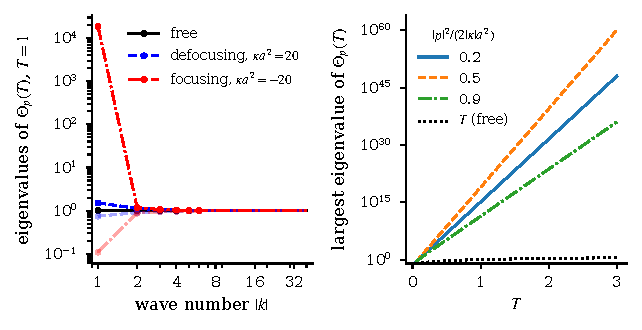
\includegraphics[width=\textwidth]{mf_nls}
\caption{Left: the two eigenvalues of the per pair information block $\Theta_p(T)$ of Proposition~\ref{m:prop:bog} at $T=1$ against the wave number $|k|$, where $|p|^2=4\pi^2|k|^2$; the larger eigenvalue is the dark curve and the smaller the pale curve of the same style. Free flow: both equal $T$. Defocusing case $\kappa a^2=20$: a compact perturbation decaying like $|p|^{-2}$, with eigenvalues $0.746$ and $1.511$ at $|k|=1$ and $0.998$ and $1.002$ at $|k|=16$. Focusing case $\kappa a^2=-20$: the mode $|k|=1$ lies inside the modulational band, $|p|^2=\lambda_1=4\pi^2<2|\kappa|a^2=40$, and its eigenvalues are $0.109$ and $1.87\times10^4$, so the larger one is amplified and the smaller one stays of order $1/(2\gamma_p)$. Right: growth in $T$ of the largest eigenvalue for $|p|^2/(2|\kappa|a^2)=0.2$, $0.5$, $0.9$ in the unstable band with $\kappa a^2=-0.6\lambda_1$ (on the unit torus only $|k|=1$ lies in this band, at the ratio $0.83$, so the three values illustrate the growth law rather than particular modes), against the free value $T$. Modulational instability amplifies the information about the initial condition exponentially along one direction, the opposite of the viscous curse of Table~\ref{m:tab:iota}.}\label{m:fig:nls}
\end{figure}

The consequences for the theory, illustrated in Figure~\ref{m:fig:nls}:
\begin{itemize}[nosep]
\item Defocusing. $\I^*_{\theta_0}\I_{\theta_0}=T\cdot\Id+\Kcal$ with $\Kcal$ block diagonal, $\norm{\Kcal_p}=O(\kappa a^2T/|p|^2)$, hence compact and two derivatives smoothing, which is the same order as in the parabolic case. Lemma~\ref{m:lem:bogmin} bounds the smallest eigenvalue of every block below, uniformly in $p$, so $\I^*_{\theta_0}\I_{\theta_0}$ is bounded above and below on $L^2$ and on every $H^\eta$, with explicit constants (Corollary~\ref{m:cor:condE}(a)). This is the analogue of Condition 2F without the factor $\Delta$, with $\eta_0=0$. The same bound is a stability estimate for the \emph{linearization} (Corollary~\ref{m:cor:condE}(b)). It is not Condition 2E, which is a lower bound on the increments of the nonlinear map $\Gcal$ and follows instead from an energy estimate for the difference of two solutions (Proposition~\ref{m:prop:nlsstab}); Remark~\ref{m:rem:condEgap} states precisely what is and is not verified. Granting the remaining conditions, the Bernstein von Mises limit is $\Ncal_{\theta_0}=N(0,T\diag\Theta_p(T)^{-1})$, whose per block covariance $T\Theta_p(T)^{-1}$ is bounded uniformly in $p$ \emph{and} in $T$ (Corollary~\ref{m:cor:condE}(c)); the limit is tight on $H^{-a}$ for $a>d/2$, and the trajectory theorem holds in weak topologies and for functionals but not in supremum norm, as in the linear case.
\item Focusing. For modes with $|p|^2<2|\kappa|a^2$ the largest eigenvalue of the block grows like $e^{2\gamma_pT}$ (Proposition~\ref{m:prop:bog}), so the component of the initial condition along the corresponding eigenvector is recovered with variance of order $Te^{-2\gamma_pT}/N$: the instability amplifies information, but along one direction of each unstable block only. The other direction is damped by the same flow, the smallest eigenvalue stays near $1/(2\gamma_p)$ (Lemma~\ref{m:lem:bogmin}(vi)), and the variance of that component is of order $2\gamma_pT/N$, which grows with $T$. There are finitely many such modes, so the tightness of the limit is not affected. The price is that the constants in Conditions 2A and 2D, which concern the nonlinear map, and the quadratic remainder of Condition 2C can be expected to grow with $T$, so that the localization set of Theorem~3 of Nickl~\cite{nicklbvm2024} would have to shrink accordingly; a Bernstein von Mises theorem can be expected only for $T$ fixed and $N\to\infty$, with constants exponential in $\gamma_{\max}T$. Computationally the curvature constant $c_{\min}$ of Nickl and Wang, the smallest eigenvalue of the normalized block $\Theta_p(T)/T$, does not become large: it is of order $1/(2\gamma_pT)$, and the amplification appears instead in the condition number $\lambda_{\max}/\lambda_{\min}$ of the block (Lemma~\ref{m:lem:bogmin}(vi)).
\item General backgrounds. For $u_0$ with several Fourier modes the conjugation term couples $p$ to $2k_0-p$ for every mode $k_0$ of $u_0$, and the time integrals in $\I^*\I$ are of the form $\int_0^Te^{i(\lambda_{p}+\lambda_{p'}-\lambda_{k_0}-\lambda_{k_0'})t}dt$: they are $O(1)$ on the four wave resonant manifold $\lambda_{k_1}+\lambda_{k_2}=\lambda_{k_3}+\lambda_{k_4}$, $k_1+k_2=k_3+k_4$, and $O(1/|\text{mismatch}|)$ off it. The resonant part is not compact in general; on $\T^2$ the resonant manifold is large. This is the structure that the wave turbulence derivation of Deng and Hani~\cite{denghani2023} exploits, and the invertibility of the information operator for a general NLS background is a question about the same resonant sums.
\item Sufficient statistic and GBC. Unchanged in form: the one step statistic \eqref{m:eq:onestep} with the adjoint of \eqref{m:eq:nlslin}, with $u_0=u_{\bar\theta_N}$. For the real inner product $\mathrm{Re}\int A\bar B$, multiplication by $i$ is skew and $U\mapsto c\bar U$ is self adjoint for every function $c$, so the adjoint of the generator $U\mapsto i\Delta U-i\kappa(2|u_0|^2U+u_0^2\bar U)$ of \eqref{m:eq:nlslin} is $W\mapsto-i\Delta W+i\kappa(2|u_0|^2W-u_0^2\bar W)$. Hence, for a source $g$ on $\mathcal X$, in \eqref{m:eq:onestep} the residuals $\sum_{i\in\mathcal I}r_i\,\delta_{X_i}$, the adjoint is $\I^*g=W(0)$, where $W$ solves the backward problem $i\partial_tW+\Delta W=\kappa(2|u_0|^2W-u_0^2\bar W)-ig$, $W(T)=0$: then $\frac{d}{dt}\mathrm{Re}\langle U,W\rangle=-\mathrm{Re}\langle U,g\rangle$ for the solution $U$ of \eqref{m:eq:nlslin}, so that $\int_0^T\mathrm{Re}\langle U(t),g(t)\rangle dt=\mathrm{Re}\langle h,W(0)\rangle$. If a Bernstein von Mises theorem holds (Remark~\ref{m:rem:condEgap}), the GBC quantile map is asymptotically affine with per pair scale $T\Theta_p(T)^{-1}/N$ about a plane wave, and a generator with $2\times2$ block structure over Fourier pairs is exact to leading order.
\end{itemize}

\subsubsection{The smallest eigenvalue of a Bogoliubov block} The blocks of Proposition~\ref{m:prop:bog} are $2\times2$, so their spectrum is determined by two scalars, and the determinant is fixed by a conservation law rather than by a computation: the Bogoliubov flow is area preserving, $\det M_p(t)=1$ for every $p$ and every $t$, in the elliptic, hyperbolic and degenerate cases alike. This is the linearized form of the conservation of the symplectic form $\mathrm{Im}\int U\bar W$ noted after \eqref{m:eq:nlslin}.

\begin{lemma}[Determinant, trace and smallest eigenvalue of $\Theta_p(T)$]\label{m:lem:bogmin}
Let $\Theta_p(T)=\int_0^TM_p(t)^\top M_p(t)\,dt$ be the block of Proposition~\ref{m:prop:bog}, and write $\omega=\omega_p$, $r=r_p=\omega_p/|p|^2$ in the elliptic case $\omega_p^2>0$, and $\gamma=\gamma_p=|\omega_p|$, $\rho=\rho_p=\gamma_p/|p|^2$ in the hyperbolic case $\omega_p^2<0$. Then, for every $T>0$:
\begin{enumerate}[label=(\roman*),nosep,leftmargin=2.2em]
\item $\det M_p(t)=1$ for all $t$, and consequently
\[
\det\Theta_p(T)\ \ge\ T^2\qquad\text{for every }p\text{ and every }T>0,
\]
with no restriction on $\omega_pT$.
\item Explicitly, for $p\ne0$ in the elliptic case,
\[
\det\Theta_p(T)=T^2+\frac{(r-r^{-1})^2}{4}\Big(T^2-\frac{\sin^2\omega T}{\omega^2}\Big),
\]
and in the hyperbolic case $\det\Theta_p(T)=T^2+\frac{(\rho+\rho^{-1})^2}{4}\big(\gamma^{-2}\sinh^2\gamma T-T^2\big)$, which is the analytic continuation $\omega\mapsto i\gamma$, $r\mapsto i\rho$ of the first formula. At $p=0$, $\Theta_0(T)=T\left(\begin{smallmatrix}1+\frac43s^2&-s\\-s&1\end{smallmatrix}\right)$ with $s=\kappa a^2T$, so $\det\Theta_0(T)=T^2(1+\tfrac13s^2)$.
\item In the elliptic case $\tr\,\Theta_p(T)=2T+(r-r^{-1})^2\int_0^T\sin^2\omega t\,dt\le T(r^2+r^{-2})$, and $\tr\,\Theta_0(T)=T(2+\tfrac43s^2)$.
\item Since $\Theta_p(T)$ is a positive definite $2\times2$ matrix, $\lambda_{\min}=\det/\lambda_{\max}\ge\det/\tr$, whence in the elliptic case
\[
\lambda_{\min}\big(\Theta_p(T)\big)\ \ge\ \frac{T}{r_p^2+r_p^{-2}},\qquad\text{and}\qquad \lambda_{\min}\big(\Theta_0(T)\big)\ \ge\ \frac T4 .
\]
If $r_p\ge1$ this implies $\lambda_{\min}\ge T/(1+r_p^2)$; if $r_p<1$ the form $T/(1+r_p^2)$ is false, so $r_p^2+r_p^{-2}$ cannot be replaced by $1+r_p^2$ in general.
\item Defocusing case, $\kappa>0$. Then $1<r_p^2\le1+2\kappa a^2/\lambda_1$ for $p\ne0$, with $\lambda_1=4\pi^2$ the smallest nonzero eigenvalue of $-\Delta$, and
\[
\begin{gathered}
\inf_p\lambda_{\min}\big(\Theta_p(T)\big)\ \ge\ \frac{T\lambda_1}{4(\lambda_1+\kappa a^2)},\\
\sup_{p\ne0}\lambda_{\max}\big(\Theta_p(T)\big)\ \le\ \frac{2T(\lambda_1+\kappa a^2)}{\lambda_1}.
\end{gathered}
\]
\item Focusing band, $\omega_p^2<0$. As $\gamma_pT\to\infty$, $\lambda_{\max}\big(\Theta_p(T)\big)\sim\tr\,\Theta_p(T)\sim(\rho_p+\rho_p^{-1})^2e^{2\gamma_pT}/(8\gamma_p)$ and $\lambda_{\min}\big(\Theta_p(T)\big)=\det\Theta_p(T)/\lambda_{\max}\to1/(2\gamma_p)$. The bound $\lambda_{\min}\ge T^2/\tr\,\Theta_p(T)$ still holds but is exponentially small in $\gamma_pT$, so it is far from sharp: the amplification is confined to one eigendirection, and the block is well conditioned in determinant and badly conditioned in ratio, with condition number $\lambda_{\max}/\lambda_{\min}\sim\frac14(\rho_p+\rho_p^{-1})^2e^{2\gamma_pT}$.
\end{enumerate}
\end{lemma}

\begin{proof}
(i) The generator $A_p$ in \eqref{m:eq:bog} has $\tr\,A_p=0$, so Liouville's formula gives $\det M_p(t)=e^{t\,\tr\,A_p}=1$. Hence $P(t):=M_p(t)^\top M_p(t)$ is symmetric positive definite with $\det P(t)=1$ for every $t$. Minkowski's determinant inequality, $\det(A+B)^{1/2}\ge(\det A)^{1/2}+(\det B)^{1/2}$ for positive semidefinite $2\times2$ matrices $A,B$, says that $P\mapsto(\det P)^{1/2}$ is superadditive on the cone; applying it to Riemann sums for $\int_0^TP(t)\,dt$ and passing to the limit,
\[
\big(\det\Theta_p(T)\big)^{1/2}\ \ge\ \int_0^T\big(\det P(t)\big)^{1/2}dt\ =\ T .
\]

(ii) to (iii) Write $C=\cos\omega t$, $S=\sin\omega t$ and
\[
\begin{gathered}
\alpha=\int_0^TC^2=\frac T2+\frac{\sin2\omega T}{4\omega},\qquad
\beta=\int_0^TS^2=\frac T2-\frac{\sin2\omega T}{4\omega},\\
\mu=\int_0^TSC=\frac{\sin^2\omega T}{2\omega},
\end{gathered}
\]
so that $\alpha+\beta=T$. By the entries of $M_p^\top M_p$ recorded in Proposition~\ref{m:prop:bog}, $\Theta_{11}=\alpha+r^2\beta$, $\Theta_{22}=\alpha+r^{-2}\beta$ and $\Theta_{12}=(r^{-1}-r)\mu$. Using $r^2+r^{-2}=2+(r-r^{-1})^2$,
\[
\begin{aligned}
\det\Theta_p&=(\alpha+r^2\beta)(\alpha+r^{-2}\beta)-(r-r^{-1})^2\mu^2\\
&=(\alpha+\beta)^2+(r-r^{-1})^2\big(\alpha\beta-\mu^2\big),
\end{aligned}
\]
and, with $\sin^22\omega T=4\sin^2\omega T\cos^2\omega T$,
\[
\begin{aligned}
\alpha\beta-\mu^2&=\frac{T^2}4-\frac{\sin^22\omega T}{16\omega^2}-\frac{\sin^4\omega T}{4\omega^2}\\
&=\frac{T^2}4-\frac{\sin^2\omega T}{4\omega^2}\big(\cos^2\omega T+\sin^2\omega T\big)
=\frac14\Big(T^2-\frac{\sin^2\omega T}{\omega^2}\Big),
\end{aligned}
\]
which is the stated determinant and, since $|\sin x|\le|x|$, recovers $\det\Theta_p\ge T^2$ with the deficit exhibited. Likewise $\tr\,\Theta_p=2\alpha+(r^2+r^{-2})\beta=2(\alpha+\beta)+(r-r^{-1})^2\beta=2T+(r-r^{-1})^2\beta$, and $\beta\le T$ gives $\tr\,\Theta_p\le T\big(2+(r-r^{-1})^2\big)=T(r^2+r^{-2})$. The hyperbolic case is the same computation with $C,S$ replaced by $\cosh\gamma t,\sinh\gamma t$. The diagonal weights of $M_p^\top M_p$ are then $\cosh^2+\rho^2\sinh^2$ and $\cosh^2+\rho^{-2}\sinh^2$, the off diagonal weight is $(\rho+\rho^{-1})\sinh\cosh$ in place of $(r^{-1}-r)\sin\cos$, and with
\[
\begin{gathered}
\alpha_h=\int_0^T\cosh^2\gamma t\,dt=\frac T2+\frac{\sinh2\gamma T}{4\gamma},\\
\beta_h=\int_0^T\sinh^2\gamma t\,dt=-\frac T2+\frac{\sinh2\gamma T}{4\gamma},\\
\mu_h=\int_0^T\sinh\gamma t\cosh\gamma t\,dt=\frac{\sinh^2\gamma T}{2\gamma}
\end{gathered}
\]
one has $\alpha_h-\beta_h=T$ in place of $\alpha+\beta=T$, $\det\Theta_p=(\alpha_h-\beta_h)^2+(\rho+\rho^{-1})^2(\alpha_h\beta_h-\mu_h^2)$, $\tr\,\Theta_p=2\alpha_h+(\rho^2+\rho^{-2})\beta_h$, and $\alpha_h\beta_h-\mu_h^2=\frac14(\gamma^{-2}\sinh^2\gamma T-T^2)\ge0$ because $\sinh x\ge x$. At $p=0$ the generator is nilpotent, $M_0(t)=\left(\begin{smallmatrix}1&0\\-2\kappa a^2t&1\end{smallmatrix}\right)$, and integrating $M_0^\top M_0$ gives the stated $\Theta_0(T)$.

(iv) For a positive definite $2\times2$ matrix, $\lambda_{\min}\lambda_{\max}=\det$ and $\lambda_{\max}\le\lambda_{\min}+\lambda_{\max}=\tr$, so $\lambda_{\min}=\det/\lambda_{\max}\ge\det/\tr$; combining (i) and (iii) gives $\lambda_{\min}\ge T^2/\big(T(r^2+r^{-2})\big)$. At $p=0$, $\det/\tr=T(3+s^2)/(6+4s^2)$, which decreases from $T/2$ at $s=0$ to $T/4$ as $s\to\infty$ and is therefore always at least $T/4$. For $r\ge1$ one has $r^{-2}\le1$, so $r^2+r^{-2}\le1+r^2$ and the weaker bound follows; for $r<1$ the inequality reverses and $T/(1+r^2)$ is not a valid bound: as $r\downarrow0$ with $|p|^2$ fixed, $M_p(t)\to\left(\begin{smallmatrix}1&|p|^2t\\0&1\end{smallmatrix}\right)$, for which $\det\Theta_p=T^2+|p|^4T^4/12$ and $\tr\,\Theta_p=2T+|p|^4T^3/3$, so $\lambda_{\min}\to T/4$ as $|p|^2T\to\infty$ while $T/(1+r^2)\to T$.

(v) In the defocusing case $r_p^2=1+2\kappa a^2/|p|^2>1$ is decreasing in $|p|$, hence $r_p^2\le R:=1+2\kappa a^2/\lambda_1$ for $p\ne0$; $x\mapsto x+x^{-1}$ is increasing on $[1,\infty)$, so $r_p^2+r_p^{-2}\le R+R^{-1}\le R+1=2(\lambda_1+\kappa a^2)/\lambda_1$, and (iv) gives $\lambda_{\min}\ge T\lambda_1/\big(2(\lambda_1+\kappa a^2)\big)$ for $p\ne0$. That exceeds $T\lambda_1/\big(4(\lambda_1+\kappa a^2)\big)$, and so does the bound $T/4$ at $p=0$ because $\lambda_1<\lambda_1+\kappa a^2$; taking the minimum over the two cases gives the first display. The second is $\lambda_{\max}\le\tr\,\Theta_p\le T(r_p^2+r_p^{-2})$ with the same estimate.

(vi) By (ii) and $\sinh^2x\sim e^{2x}/4$, $\det\Theta_p(T)\sim(\rho+\rho^{-1})^2e^{2\gamma T}/(16\gamma^2)$, and since $\alpha_h,\beta_h\sim e^{2\gamma T}/(8\gamma)$, $\tr\,\Theta_p(T)=2\alpha_h+(\rho^2+\rho^{-2})\beta_h\sim(2+\rho^2+\rho^{-2})e^{2\gamma T}/(8\gamma)=(\rho+\rho^{-1})^2e^{2\gamma T}/(8\gamma)$. Hence $\det/\tr\to1/(2\gamma)$ and $\det/\tr^2\to0$, and from $\lambda_{\min}=2\det/\big(\tr+\sqrt{\tr^2-4\det}\big)$ we get $\lambda_{\min}=(\det/\tr)(1+o(1))\to1/(2\gamma)$ and $\lambda_{\max}=\tr\,(1+o(1))$. The condition number is $\lambda_{\max}/\lambda_{\min}=\lambda_{\max}^2/\det\sim\frac14(\rho+\rho^{-1})^2e^{2\gamma T}$.
\end{proof}

If observation starts at $T_0>0$, the information on $[T_0,T]$ is $\int_{T_0}^TM_p^\top M_p\,dt$, and Lemma~\ref{m:lem:bogmin} says what survives. For a stable mode with $p\ne0$ the proofs of (i), (iii) and (iv) use only $\det M_p(t)=1$ and the pointwise bound $\tr\big(M_p(t)^\top M_p(t)\big)\le r_p^2+r_p^{-2}$, so the bounds hold with $T$ replaced by $T-T_0$: the position of the window does not enter them, as in the linear case. Two things change. In the focusing band the damped eigenvector $v$ of $A_p$ satisfies $M_p(t)v=e^{-\gamma_pt}v$, so the Rayleigh quotient gives $\lambda_{\min}\big(\int_{T_0}^TM_p^\top M_p\,dt\big)\le e^{-2\gamma_pT_0}/(2\gamma_p)$: a late window loses the information along the damped direction, as in the dissipation barrier of Table~\ref{m:tab:iota}, but for the finitely many unstable modes only (for $\kappa a^2=-20$, $|k|=1$ and windows of length one the bound is sharp to within one percent). At $p=0$ the shear $M_0(t)$ grows linearly: with $\tau=T-T_0$ the window block has determinant $\tau^2\big(1+\tfrac13\kappa^2a^4\tau^2\big)$ and trace $\tau\big(2+\tfrac43\kappa^2a^4(T^2+TT_0+T_0^2)\big)$, so its smallest eigenvalue decays like $T_0^{-2}$, for the single mode $p=0$.

\begin{corollary}[Linearized stability and the analogue of Condition 2F for the defocusing plane wave]\label{m:cor:condE}
Let $\kappa>0$, $\theta_0=a$ constant, and let $\I_{\theta_0}$ be the linearization \eqref{m:eq:nlslin}, with adjoint taken with respect to unnormalized $L^2(\mathcal X)$, $\mathcal X=[0,T]\times\T^d$. Set
\[
c_\star^2=\frac{T\lambda_1}{4(\lambda_1+\kappa a^2)},\qquad
C_\star^2=\max\Big\{\frac{2T(\lambda_1+\kappa a^2)}{\lambda_1},\ T\big(2+\tfrac43\kappa^2a^4T^2\big)\Big\}.
\]
Then for every $h\in L^2(\T^d;\C)$,
\[
c_\star^2\norm{h}_{L^2(\Omega)}^2\ \le\ \norm{\I_{\theta_0}h}^2_{L^2(\mathcal X)}=\big\langle h,\I^*_{\theta_0}\I_{\theta_0}h\big\rangle\ \le\ C_\star^2\norm{h}_{L^2(\Omega)}^2,
\]
and consequently
\begin{enumerate}[label=(\alph*),nosep,leftmargin=2.2em]
\item $\I^*_{\theta_0}\I_{\theta_0}$ is a homeomorphism of $H^\eta(\T^d)$ for every $\eta\in\R$, with the explicit constants $c_\star^2,C_\star^2$; this is the analogue of Condition 2F without the factor $\Delta$, with $\eta_0=0$, and no smoothing is needed, while Condition 2F as stated fails, since $\Delta\I^*_{\theta_0}\I_{\theta_0}$ loses two derivatives;
\item the linearization satisfies the stability estimate
\[
\norm{\I_{\theta_0}h}_{L^2(\mathcal X)}\ \ge\ c_\star\norm{h}_{L^2(\Omega)}\ \ge\ c_\star\norm{h}_{H^{-1}(\Omega)} ,
\]
which is the estimate of Condition 2E with $\I_{\theta_0}$ in place of $\Gcal$, in the stronger norm $L^2$ rather than $H^{-1}$;
\item $\Ncal_{\theta_0}=N\big(0,T(\I^*_{\theta_0}\I_{\theta_0})^{-1}\big)=N\big(0,T\diag\Theta_p(T)^{-1}\big)$ has per block covariance $T\Theta_p(T)^{-1}$ with
\[
\norm{T\Theta_p(T)^{-1}}\ \le\ \frac{T}{\lambda_{\min}(\Theta_p(T))}\ \le\ \frac{4(\lambda_1+\kappa a^2)}{\lambda_1}
\]
uniformly in $p$ and in $T$, so $\Ncal_{\theta_0}$ is tight on $H^{-a}$ for $a>d/2$; contrast the parabolic case, where $1/\iota_j\asymp2\nu\lambda_jT$ diverges with $j$ and with $T$.
\end{enumerate}
\end{corollary}

\begin{proof}
The Bogoliubov substitution $U=e^{-i\kappa a^2t}(\phi+i\psi)$ is at each $t$ a pointwise rotation of $\C\cong\R^2$, hence an isometry of $L^2(\T^d;\C)$, and $\norm{h}^2_{L^2(\Omega)}=\norm{\phi(0)}^2+\norm{\psi(0)}^2$ for $h=U(0)$, the norms being those of the real functions $\phi(0),\psi(0)$. Because the design is uniform on $\mathcal X$, whose measure is $T$, and the adjoint is unnormalized,
\[
\begin{aligned}
\norm{\I_{\theta_0}h}^2_{L^2(\mathcal X)}&=\int_0^T\norm{U(t)}^2_{L^2(\T^d)}dt=\sum_p\int_0^T\big|M_p(t)v_p\big|^2dt\\
&=\sum_p\big\langle v_p,\Theta_p(T)v_p\big\rangle,\qquad v_p=\big(\phi_p(0),\psi_p(0)\big),
\end{aligned}
\]
with $\sum_p|v_p|^2=\norm{h}^2_{L^2(\Omega)}$ by Parseval. The two sided bound is Lemma~\ref{m:lem:bogmin}(v) applied term by term, together with $\lambda_{\max}(\Theta_0(T))\le\tr\,\Theta_0(T)=T(2+\frac43\kappa^2a^4T^2)$ for the zero mode. For (a), each block acts within a single $p$ and therefore commutes with the Sobolev weights $(1+\lambda_p)^{\eta/2}$, so the two sided bound on $L^2$ transfers to $H^\eta$ for every $\eta$. Part (b) is the left inequality together with $\norm{h}_{H^{-1}}\le\norm{h}_{L^2}$. Part (c) is the block inverse, with tightness as in Proposition~\ref{m:prop:sch}: $\sum_p\lambda_p^{-a}<\infty$ for $a>d/2$.
\end{proof}

The stability estimate for $\Gcal$ itself does not go through the linearization.

\begin{proposition}[Stability of the cubic NLS solution map]\label{m:prop:nlsstab}
Let $\kappa\ne0$, let $u$ and $v$ solve $i\partial_tu+\Delta u=\kappa|u|^2u$ on $[0,T]\times\T^d$ with data $\theta$ and $\vartheta$, in $H^1$ if $d=1$ and in $H^2$ if $d=2$, and suppose that $\norm{u(t)}_{L^\infty}\le M_\infty$ and $\norm{v(t)}_{L^\infty}\le M_\infty$ for $t\le T$, with $M_\infty>0$. Then, for $t\le T$,
\[
e^{-6|\kappa|M_\infty^2t}\norm{\theta-\vartheta}^2_{L^2(\Omega)}\ \le\ \norm{u(t)-v(t)}^2_{L^2(\Omega)}\ \le\ e^{6|\kappa|M_\infty^2t}\norm{\theta-\vartheta}^2_{L^2(\Omega)},
\]
and, with the unnormalized $L^2(\mathcal X)$ of Corollary~\ref{m:cor:condE},
\[
\begin{aligned}
\norm{\Gcal(\theta)-\Gcal(\vartheta)}^2_{L^2(\mathcal X)}&\ge\frac{1-e^{-6|\kappa|M_\infty^2T}}{6|\kappa|M_\infty^2}\norm{\theta-\vartheta}^2_{L^2(\Omega)}\\
&\ge Te^{-6|\kappa|M_\infty^2T}\norm{\theta-\vartheta}^2_{H^{-1}(\Omega)} .
\end{aligned}
\]
A bound $M_\infty=M_\infty(T,\kappa,B)$ that holds for all data in a ball of radius $B$ exists in each of the following cases:
\begin{enumerate}[label=(\alph*),nosep,leftmargin=2.2em]
\item $d=1$, either sign of $\kappa$, every ball of $H^1$;
\item $d=2$, $\kappa>0$, every ball of $H^2$;
\item $d=2$, $\kappa<0$, the balls of $H^2$ with $2|\kappa|C_2B^2T<1$, where $C_2$ is a constant such that $\norm{|f|^2f}_{H^2}\le C_2\norm f^3_{H^2}$.
\end{enumerate}
On such a ball, Condition 2E therefore holds for $\Gcal$, with the stronger norm $L^2$ on the right and the constant $T^{1/2}e^{-3|\kappa|M_\infty^2T}$, Condition 2A holds with the bound $M_\infty$, and the upper bound gives the $L^2$ Lipschitz estimate of Condition 2B, $\norm{\Gcal(\theta)-\Gcal(\vartheta)}^2_{L^2(\mathcal X)}\le\big(e^{6|\kappa|M_\infty^2T}-1\big)\norm{\theta-\vartheta}^2_{L^2(\Omega)}/(6|\kappa|M_\infty^2)$.
\end{proposition}

\begin{proof}
Write $f(z)=|z|^2z$ and $w=u-v$. Since $|\partial_zf|+|\partial_{\bar z}f|=3|z|^2$, pointwise
\[
|f(u)-f(v)|\ \le\ 3|w|\int_0^1|v+sw|^2ds\ \le\ \tfrac32\big(|u|^2+|v|^2\big)|w| .
\]
The difference solves $\partial_tw=i\Delta w-i\kappa\big(f(u)-f(v)\big)$, and $i\Delta$ is skew for the real inner product $\mathrm{Re}\langle\cdot,\cdot\rangle$ of $L^2(\Omega)$, so
\[
\Big|\frac d{dt}\norm{w}^2_{L^2(\Omega)}\Big|=2|\kappa|\,\big|\mathrm{Re}\big\langle f(u)-f(v),iw\big\rangle\big|\le6|\kappa|M_\infty^2\norm{w}^2_{L^2(\Omega)},
\]
and Gr\"onwall's inequality, forward and backward in time, gives the two sided bound. For the uniform design $\norm{\Gcal(\theta)-\Gcal(\vartheta)}^2_{L^2(\mathcal X)}=\int_0^T\norm{w(t)}^2_{L^2(\Omega)}dt$, so integrating the lower bound gives the first inequality of the second display, $(1-e^{-x})/x\ge e^{-x}$ and $\norm\cdot_{H^{-1}}\le\norm\cdot_{L^2}$ give the second, and integrating the upper bound gives the Lipschitz estimate.

(a) The mass $m=\norm{u(t)}^2_{L^2}$ and the energy $E=\norm{\partial_xu(t)}^2_{L^2}+\frac\kappa2\norm{u(t)}^4_{L^4}$ do not depend on $t$, and on the circle of length one $\norm g^2_{L^\infty}\le\norm g^2_{L^2}+2\norm g_{L^2}\norm{\partial_xg}_{L^2}$, so that $m$ and $E$ are bounded on the ball. If $\kappa>0$, then $\norm{\partial_xu(t)}^2_{L^2}\le E$. If $\kappa<0$, the same inequality gives $\norm{u}^4_{L^4}\le\norm u^2_{L^\infty}\norm u^2_{L^2}\le m^2+2m^{3/2}\norm{\partial_xu}_{L^2}$, so $y=\norm{\partial_xu(t)}_{L^2}$ satisfies $y^2\le E+|\kappa|(m^2/2+m^{3/2}y)$, a quadratic inequality that bounds $y$. In both cases $\norm{u(t)}_{H^1}$ is bounded for all $t$ by a function of $B$ and $\kappa$, which also continues the local solution to all times, and the inequality above bounds $\norm{u(t)}_{L^\infty}$. (b) Since $\sqrt\kappa\,u$ solves $i\partial_tu+\Delta u=|u|^2u$, Theorem~1.1 of Planchon, Tzvetkov and Visciglia~\cite{ptv2017}, applied to the $H^2$ norm, bounds $\sup_{t\le T}\norm{u(t)}_{H^2}$ in terms of $T$ and $\norm\theta_{H^2}$ (their argument also gives the global existence that the theorem assumes), and $H^2(\T^2)\subset L^\infty$. (c) Since $i\Delta$ commutes with $1-\Delta$, it is skew in $H^2$ as well, and $y(t)=\norm{u(t)}^2_{H^2}$ satisfies $y'\le2|\kappa|\norm{f(u)}_{H^2}\norm u_{H^2}\le2|\kappa|C_2y^2$; hence $y(t)\le y(0)/(1-2|\kappa|C_2y(0)t)\le B^2/(1-2|\kappa|C_2B^2T)$ on $[0,T]$, which also continues the local solution to $[0,T]$, and again $H^2(\T^2)\subset L^\infty$.
\end{proof}

\begin{remark}[What is verified, what is not, and what would close the gap]\label{m:rem:condEgap}
Condition 2E, as recorded in Section~\ref{m:sec:papers}, is the estimate $\norm{\Gcal(\theta)-\Gcal(\theta_0)}_{L^2(\mathcal X)}\ge c\norm{\theta-\theta_0}_{H^{-1}}$ for the \emph{nonlinear} solution map $\Gcal$, required uniformly over the Sobolev ball supporting the prior. Corollary~\ref{m:cor:condE}(b) is that estimate for $\I_{\theta_0}=D\Gcal_{\theta_0}$, the derivative at a single point. The two statements are different and neither implies the other; the second is a local injectivity and curvature statement about the tangent space of the solution manifold at $u_{\theta_0}$, not an identifiability statement about $\Gcal$.

Three things separate them. First, the passage from the derivative to the secant is only local. Along the segment $\vartheta_s=\theta_0+s(\theta-\theta_0)$,
\[
\begin{aligned}
\Gcal(\theta)-\Gcal(\theta_0)&=\int_0^1\I_{\vartheta_s}(\theta-\theta_0)\,ds\\
&=\I_{\theta_0}(\theta-\theta_0)+\int_0^1\big(\I_{\vartheta_s}-\I_{\theta_0}\big)(\theta-\theta_0)\,ds ,
\end{aligned}
\]
so if the linearization were Lipschitz in its base point, $\norm{(\I_\vartheta-\I_{\theta_0})h}_{L^2(\mathcal X)}\le L\norm{\vartheta-\theta_0}_{H^\zeta}\norm{h}_{L^2}$ for some $\zeta>d/2$ and all $\vartheta$ on the segment, then Corollary~\ref{m:cor:condE}(b) would give
\[
\norm{\Gcal(\theta)-\Gcal(\theta_0)}_{L^2(\mathcal X)}\ \ge\ \Big(c_\star-\tfrac L2\norm{\theta-\theta_0}_{H^\zeta}\Big)\norm{\theta-\theta_0}_{L^2(\Omega)} ,
\]
that is, Condition 2E with constant $c_\star/2$ and with the stronger norm $L^2$ on the right, but only on $\{\norm{\theta-\theta_0}_{H^\zeta}\le c_\star/L\}$. Nothing above bounds $L$ for cubic NLS; $L$ depends on $T$ and on $\norm{\theta}_{H^\zeta}$, and in the focusing band the linearized flow itself varies on the scale $e^{\gamma_{\max}T}$, so such a radius can be expected to shrink exponentially in $T$.

Second, a local estimate is not Condition 2E. Condition 2E is global on the ball, and it is what excludes a second $\theta$ far from $\theta_0$ with $\Gcal(\theta)$ close to $\Gcal(\theta_0)$. For cubic NLS the global statement does not need the linearization: it is Proposition~\ref{m:prop:nlsstab}, on every ball on which the solutions stay bounded, which for $d\le2$ and $\kappa>0$ is every ball of $H^2$. The reason is the reverse of the parabolic one. The flow is unitary on $L^2$ and the nonlinearity is Lipschitz on bounded sets, so two solutions approach each other at most exponentially fast and the distance between their initial data is never lost, only reduced by the factor $e^{-3|\kappa|M_\infty^2t}$. For the heat equation and Navier Stokes the semigroup damps differences, which is why the right side of Condition 2E carries the weaker norm $H^{-1}$ there, by \eqref{m:eq:modeinfo} and by Konen and Nickl~\cite{konennickl2026} respectively.

Third, even the derivative estimate is proved only at the plane wave background. For a general $\theta_0$, $\I^*_{\theta_0}\I_{\theta_0}$ is no longer block diagonal, and its invertibility is the four wave resonant sum question of the third bullet above and of Open Question~\ref{m:op:planewave} below. The segment $\vartheta_s$ passes through such backgrounds even when both endpoints are plane waves, as soon as their wave vectors differ, so the first point above cannot be run at the plane wave alone.

The accounting for cubic NLS about a plane wave in the defocusing case is therefore: the analogue of Condition 2F without the factor $\Delta$ is verified with $\eta_0=0$ and explicit constants (Corollary~\ref{m:cor:condE}(a)), and Condition 2F itself fails, as for the linear equation; the linearized stability estimate is verified in $L^2$, hence a fortiori in $H^{-1}$ (Corollary~\ref{m:cor:condE}(b)); Condition 2E for $\Gcal$ is verified in $L^2$ on every ball of $H^2$, for $d\le2$, together with Condition 2A and the $L^2$ Lipschitz estimate of Condition 2B (Proposition~\ref{m:prop:nlsstab}); Conditions 2C and 2D are \emph{not} verified. Closing the gap requires the estimates of Conditions 2C and 2D, in particular a bound on the Lipschitz modulus of $\theta\mapsto\I_\theta$ from $H^\zeta$ into $\mathcal B\big(L^2(\Omega),L^2(\mathcal X)\big)$ on the localization set, which is a well posedness estimate for \eqref{m:eq:nlslin} with variable background, and a version of Theorem~\ref{m:thm:nickl2} under the analogue of Condition 2F without the factor $\Delta$.
\end{remark}


\subsection{The examples side by side}

Tables~\ref{m:tab:compare} and~\ref{m:tab:guarantee} collect the objects of Sections~\ref{m:sec:suff} to~\ref{m:sec:nondiss} for the heat equation, two dimensional Navier Stokes about the Taylor Green vortex, and the linear and cubic Schr\"odinger equations. The two dissipative columns differ only by a compact perturbation; the two dispersive columns differ from them in every row that involves smoothing or forgetting.

\begin{table}[tp]\centering\scriptsize
\setlength{\tabcolsep}{2pt}
\caption{Objects of the theory for the four examples, part one: the forward map, the information operator and the summary. $\lambda_j=4\pi^2|k_j|^2$; $\Theta_p(T)$ the Bogoliubov information block of Proposition~\ref{m:prop:bog}; $\Kcal$ compact. The $\I^*\I$ row is unnormalized ($\int_0^T$, as in \eqref{m:eq:modeinfo}) while $\iota_j$ is normalized ($\tfrac1T\int_0^T$, as in \eqref{m:eq:iota}). For cubic NLS the per mode information is the pair of eigenvalues of $T^{-1}\Theta_p(T)$, and the quantile map of the last row is conditional on a Bernstein von Mises theorem, which is not proved here (Remark~\ref{m:rem:condEgap}).}\label{m:tab:compare}
\begin{tabular}{>{\raggedright\arraybackslash}p{0.155\textwidth}>{\raggedright\arraybackslash}p{0.175\textwidth}>{\raggedright\arraybackslash}p{0.21\textwidth}>{\raggedright\arraybackslash}p{0.15\textwidth}>{\raggedright\arraybackslash}p{0.235\textwidth}}
\toprule
& Heat & Two dimensional Navier Stokes (Taylor Green) & Linear Schr\"odinger & Cubic NLS (plane wave)\\
\midrule
Forward map & $e^{\nu t\Delta}$ & nonlinear; $u_{\rm TG}$ exact & $e^{it\Delta}$, unitary & nonlinear, preserves the $L^2$ norm\\
Linearization $\I_{\theta_0}$ & $e^{\nu t\Delta}$ & Stokes $+$ nearest neighbor coupling $A|k|e^{-2\nu t}$ & $e^{it\Delta}$ itself & Bogoliubov $2\times2$ blocks \eqref{m:eq:bog}\\
$\I^*\I$ & $\diag(T\iota_j)$ & $\Lcal^*\Lcal+\Kcal$, $\Delta\Lcal^*\Lcal=(S_{2T}-\Id)/(2\nu)$ & $T\cdot\Id$ exactly & $\diag(\Theta_p(T))$, Prop.~\ref{m:prop:bog}\\
Per mode information & $\iota_j\asymp(2\nu\lambda_jT)^{-1}$ & same $+O\big(A/(\nu|k|)\big)$ & $1$ & defocusing: $1+O(\kappa a^2/|p|^2)$; focusing band: largest eigenvalue grows like $e^{2\gamma_pT}$, smallest is $\sim1/(2\gamma_pT)$\\
Effect of $T_0>0$ & factor $e^{-2\nu\lambda_jT_0}$ & same & none & no decay for stable modes with $p\ne0$; focusing band: damped direction at most $e^{-2\gamma_pT_0}/(2\gamma_p)$; $p=0$: smallest eigenvalue decays like $T_0^{-2}$, after Lem.~\ref{m:lem:bogmin}\\
Sufficient statistic & adjoint heat flow of data, exact & one step efficient score via adjoint linearized Navier Stokes & adjoint unitary flow of data, exact & one step efficient score via $W(0)$, with $W$ the backward solution of the adjoint of \eqref{m:eq:nlslin}\\
GBC quantile map & affine, scale $(N\iota_j+\rho^{-2}\lambda_j^\alpha)^{-1/2}$ for the limit Gram matrix $N\diag(\iota_j)$ & asymptotically affine, scale $T(\I^*\I)^{-1}/N$ & affine, scale $(N+\rho^{-2}\lambda_j^\alpha)^{-1/2}$ for the limit Gram matrix $N\,\Id$ & asymptotically affine, $2\times2$ block scale $T\Theta_p(T)^{-1}/N$\\
\bottomrule
\end{tabular}
\end{table}

\begin{table}[tp]\centering\scriptsize
\setlength{\tabcolsep}{2pt}
\caption{Objects of the theory for the four examples, part two: the limit theorems and the conditions. BvM stands for Bernstein von Mises. As in Table~\ref{m:tab:compare}, $\I^*\I$ is unnormalized and $\iota_j$ normalized, so that $\Ncal_{\theta_0}=N(0,T(\I^*\I)^{-1})=N(0,\diag(1/\iota_j))$ in every column; for cubic NLS $c_{\min}$ is the smallest eigenvalue of $T^{-1}\Theta_p(T)$ over the modes retained. The row on $c_{\min}$ gives the value of the curvature constant of the localized Langevin algorithm of Nickl and Wang~\cite{nicklwang2024} if their remaining conditions carry over (Section~\ref{sec:gradstab}). $^\dagger$For cubic NLS no Bernstein von Mises theorem is proved here: Conditions 2C and 2D are not verified, and Condition 2F holds only without the factor $\Delta$ (Remark~\ref{m:rem:condEgap}); Section~\ref{m:sec:nondiss} notes that the theorem can be expected for $T$ fixed.}\label{m:tab:guarantee}
\begin{tabular}{>{\raggedright\arraybackslash}p{0.155\textwidth}>{\raggedright\arraybackslash}p{0.175\textwidth}>{\raggedright\arraybackslash}p{0.21\textwidth}>{\raggedright\arraybackslash}p{0.15\textwidth}>{\raggedright\arraybackslash}p{0.235\textwidth}}
\toprule
& Heat & Two dimensional Navier Stokes (Taylor Green) & Linear Schr\"odinger & Cubic NLS (plane wave)\\
\midrule
BvM limit $\Ncal_{\theta_0}$ & $N(0,\diag(1/\iota_j))$ & $N(0,T(\I^*\I)^{-1})$ & $N(0,\Id)$ & $N(0,T\diag\Theta_p(T)^{-1})$\\
Tight on & $H^{-a}$, $a>1+d/2$ & $\Hds{-\beta}$, $\beta>2$ & $H^{-a}$, $a>d/2$ & $H^{-a}$, $a>d/2$\\
Trajectory BvM in sup norm & yes, $t>0$ & yes, $t>0$ & no & no\\
Trajectory BvM, weak topology & yes & yes & yes, Cor.~\ref{m:cor:schtransfer}(ii) & conjectural$^\dagger$\\
Functionals efficient at rate $\sqrt N$ & yes & yes & yes, Cor.~\ref{m:cor:schtransfer}(iv) & conjectural$^\dagger$ ($T$ fixed)\\
Nickl Wang $c_{\min}$, if the remaining conditions hold & $\min_j\iota_j\asymp D^{-2/d}$ & same & $1$ & defocusing: at least $\frac{\lambda_1}{4(\lambda_1+\kappa a^2)}$, uniformly in $D$ and $T$; focusing band: $\sim1/(2\gamma_pT)$\\
Condition 2E verified & yes, $\Gcal$ linear, \eqref{m:eq:modeinfo} gives it in $H^{-1}$ & Konen Nickl & yes, $\Gcal$ linear, in $L^2$ & yes, in $L^2$, on balls where the solutions stay bounded, which for $\kappa>0$ is every $H^2$ ball, Prop.~\ref{m:prop:nlsstab}; linearized form, Cor.~\ref{m:cor:condE}(b)\\
Condition 2F verified & trivially & Konen Nickl & fails; holds without the factor $\Delta$, as $\I^*\I=T\cdot\Id$ & fails; without the factor $\Delta$: plane wave, defocusing, Lem.~\ref{m:lem:bogmin}, Cor.~\ref{m:cor:condE}(a); general: open (resonances)\\
\bottomrule
\end{tabular}
\end{table}

\begin{proposition}[Linear Schr\"odinger transfer]\label{m:prop:sch}
For the linear Schr\"odinger equation, let the noise have independent standard Gaussian real and imaginary parts, let the prior be \eqref{m:eq:prior} truncated to the first $D=D_N$ modes, so that the real and the imaginary part of $\theta_j$ are independent with precision $\rho^{-2}\lambda_j^\alpha$, where $\rho^{-2}=N\delta_N^2$, $\alpha=\gamma$ and $\gamma>d/2$, let $\tilde\theta_N$ be the posterior mean, and write $N(0,\Id)$ for complex white noise whose real and imaginary parts are independent with covariance $\Id$. Then:
\begin{enumerate}[label=(\alph*),nosep,leftmargin=2.2em]
\item the posterior is exactly Gaussian, the adjoint summary $\Phi^*Y$ together with the design is exactly sufficient, and the GBC quantile map is exactly affine, with per mode scale $(N+\rho^{-2}\lambda_j^\alpha)^{-1/2}$ in the real and in the imaginary part when the Gram matrix $\Phi^*\Phi$ of the design is replaced by its limit $N\,\Id$;
\item if $D_N\to\infty$ and $D_N=o(N^{d/(2\gamma+d)})$, then $\Wone_{1,H^{-a}}\big(\Law(\sqrt N(\theta-\tilde\theta_N)\mid Z^{(N)}),N(0,\Id)\big)\to^P0$ for every $a>d/2$;
\item if in addition $\theta_0\in H^\gamma$ and $N\lambda_{D_N}^{-(a+\gamma)}\to0$, then $\sqrt N(\tilde\theta_N-\theta_0)\to^dN(0,\Id)$ in $H^{-a}$; the choice $D_N\asymp N^{d/(2\gamma+d)}/\log N$ meets the conditions of (b) and (c) for every $a>d/2$;
\item (b) and (c) hold with $u_\theta(t)$, $u_{\tilde\theta_N}(t)$ and $u_{\theta_0}(t)$ in place of $\theta$, $\tilde\theta_N$ and $\theta_0$, at every $t$ and uniformly in $t$, with the same limit $e^{it\Delta}_\#N(0,\Id)=N(0,\Id)$, and no supremum norm statement holds at any $t$.
\end{enumerate}
\end{proposition}

\begin{proof}
Write $\phi_i=\big(e^{i\lambda_jt_i}\overline{e_j(x_i)}\big)_{j\le D}$, so that $\Phi^*\Phi=\sum_i\phi_i\phi_i^*$ and $\Phi^*Y=\sum_i\phi_iY_i$, let $V_N=(\Phi^*\Phi+\rho^{-2}\Lambda^\alpha)^{-1}$, and let $P_D$ be the projection on the first $D$ modes.

(a) Up to a constant the log posterior density is $-\frac12(\theta-V_N\Phi^*Y)^*V_N^{-1}(\theta-V_N\Phi^*Y)$, so, as in Proposition~\ref{m:prop:linsuff}, the posterior is Gaussian with mean $\tilde\theta_N=V_N\Phi^*Y$, it depends on the data only through $\Phi^*Y$ and the design, and the real and imaginary parts of $\theta$ have the joint covariance $\left(\begin{smallmatrix}\mathrm{Re}V_N&-\mathrm{Im}V_N\\\mathrm{Im}V_N&\mathrm{Re}V_N\end{smallmatrix}\right)$. The real and the imaginary part of $\theta_j$ therefore have posterior variance $(V_N)_{jj}$, which is $(N+\rho^{-2}\lambda_j^\alpha)^{-1}$ when $\Phi^*\Phi=N\,\Id$, and the quantile map is that of \eqref{m:eq:linquant}.

(b) The $\phi_i$ are independent, their entries have modulus one, and $E[\phi_i\phi_i^*]=\Id$ because the $e_j$ are orthonormal and $x_i$ is uniform. The matrices $S_i=N^{-1}(\phi_i\phi_i^*-\Id)$ are centered, with $\norm{S_i}\le D/N$ and $\sum_iE[S_i^2]=N^{-1}(D-1)\Id$, so the matrix Bernstein inequality, Theorem~6.1.1 of Tropp~\cite{tropp2015}, gives for $\Gamma=N^{-1}\Phi^*\Phi-\Id$
\[
E\norm\Gamma\le\sqrt{\frac{2D\log(2D)}N}+\frac{D\log(2D)}{3N},
\]
which tends to zero because $D\log D=o(N)$. With $\Lambda_\delta=\delta_N^2\Lambda^\gamma=N^{-1}\rho^{-2}\Lambda^\alpha$ on the first $D$ modes, $NV_N=(\Id+\Lambda_\delta+\Gamma)^{-1}$ and $\Id+\Lambda_\delta\succeq\Id$, so on $\{\norm\Gamma<1\}$
\[
\norm{NV_N}\le\frac1{1-\norm\Gamma},\qquad\norm{NV_N-\Id}\le\frac{\norm\Gamma+\norm{\Lambda_\delta}}{1-\norm\Gamma},
\]
and $\norm{\Lambda_\delta}=\delta_N^2\lambda_D^\gamma\to0$ exactly when $D=o(N^{d/(2\gamma+d)})$, since $\lambda_D\asymp D^{2/d}$. Let $G$ have law $N(0,\Id)$. Then $(NV_N)^{1/2}P_DG$ has the posterior law of $\sqrt N(\theta-\tilde\theta_N)$, and for a matrix $A$ acting on the first $D$ modes $E\norm{AG}^2_{H^{-a}}=2\sum_j\lambda_j^{-a}(AA^*)_{jj}\le2\norm A^2\sum_{j\le D}\lambda_j^{-a}$. With $|\sqrt\mu-1|\le|\mu-1|$ for $\mu\ge0$, the square of the distance in (b) is therefore at most
\[
E\norm{(NV_N)^{1/2}P_DG-G}^2_{H^{-a}}\le2\norm{NV_N-\Id}^2\sum_j\lambda_j^{-a}+2\sum_{j>D}\lambda_j^{-a},
\]
which tends to zero in probability, because $\sum_j\lambda_j^{-a}<\infty$ for $a>d/2$.

(c) Write $Y=\Phi P_D\theta_0+r+\varepsilon$, where $r_i=u_{\theta_0-P_D\theta_0}(t_i,x_i)$ is the signal of the modes above $D$. Since $V_N\Phi^*\Phi=\Id-(NV_N)\Lambda_\delta$,
\[
\begin{aligned}
\sqrt N(\tilde\theta_N-\theta_0)&=\sqrt NV_N\Phi^*\varepsilon-\sqrt N(NV_N)\Lambda_\delta P_D\theta_0\\
&\quad+\sqrt NV_N\Phi^*r-\sqrt N(\theta_0-P_D\theta_0),
\end{aligned}
\]
and we take the four terms in turn; the norm of $H^{-a}$ is at most $\lambda_1^{-a/2}$ times that of $L^2$. Given the design, the first term is centered Gaussian, with the covariance structure of (a) for the matrix $(NV_N)(\Id+\Gamma)(NV_N)$, which tends to $\Id$ in operator norm, so the coupling of (b) shows that its law tends to $N(0,\Id)$ in $\Wone_{1,H^{-a}}$. In the second, $(NV_N)\Lambda_\delta=(\Id+\Lambda_\delta)^{-1}\Lambda_\delta-(NV_N)\Gamma(\Id+\Lambda_\delta)^{-1}\Lambda_\delta$. For the diagonal part, $b/(1+b)\le\min(1,b)\le b^{(a+\gamma)/(2\gamma)}$ for $b\ge0$ and $d/2<a\le\gamma$, so
\[
\begin{aligned}
N\norm{(\Id+\Lambda_\delta)^{-1}\Lambda_\delta P_D\theta_0}^2_{H^{-a}}&\le N\sum_j\lambda_j^{-a}\big(\delta_N^2\lambda_j^\gamma\big)^{(a+\gamma)/\gamma}|\theta_{0,j}|^2\\
&\le N\delta_N^{2(a+\gamma)/\gamma}\norm{\theta_0}^2_{H^\gamma},
\end{aligned}
\]
and $N\delta_N^{2(a+\gamma)/\gamma}=N^{(d-2a)/(2\gamma+d)}\to0$; for $a>\gamma$ the norm of $H^{-a}$ is weaker and the bound at $a=\gamma$ applies. For the rest of the second term, $(b/(1+b))^2\le b$ gives $\norm{(\Id+\Lambda_\delta)^{-1}\Lambda_\delta P_D\theta_0}_{L^2}\le\delta_N\norm{\theta_0}_{H^\gamma}$, so its contribution is $O_P(\sqrt N\norm\Gamma\delta_N)=O_P(\delta_N\sqrt{D\log D})$, which tends to zero because $D\delta_N^2\le N^{(d-2\gamma)/(2\gamma+d)}$ eventually and $\gamma>d/2$. In the third, the vectors $\phi_ir_i$ are independent and centered, because $e_j$, $j\le D$, is orthogonal in $L^2(\T^d)$ to every mode of $r$, and $E\norm{\phi_ir_i}^2=D\norm{\theta_0-P_D\theta_0}^2_{L^2}$; hence $\sqrt N\norm{V_N\Phi^*r}_{L^2}\le\norm{NV_N}\sqrt N\norm{N^{-1}\Phi^*r}=O_P\big(\sqrt D\lambda_D^{-\gamma/2}\big)\norm{\theta_0}_{H^\gamma}=O_P(D^{1/2-\gamma/d})$, which tends to zero. The last term satisfies $N\norm{\theta_0-P_D\theta_0}^2_{H^{-a}}\le N\lambda_D^{-(a+\gamma)}\norm{\theta_0}^2_{H^\gamma}\to0$, and Slutsky's lemma gives (c). For $D_N\asymp N^{d/(2\gamma+d)}/\log N$, $D_N=o(N^{d/(2\gamma+d)})$, and $N\lambda_{D_N}^{-(a+\gamma)}$ is $N^{(d-2a)/(2\gamma+d)}$ times a power of $\log N$, which tends to zero for every $a>d/2$.

(d) The operator $e^{it\Delta}$ multiplies mode $j$ by $e^{-i\lambda_jt}$, so it is an isometry of every $H^s$ that maps $N(0,\Id)$ to itself, and $u_\theta(t)-u_{\vartheta}(t)=e^{it\Delta}(\theta-\vartheta)$; Wasserstein and bounded Lipschitz distances between laws on $H^{-a}$ are therefore the same at every $t$ as at $t=0$. Failure in supremum norm: $N(0,\Id)$ is not tight in $C(\T^d)$, and $e^{it\Delta}$ preserves this.
\end{proof}

\begin{corollary}[The transfer theorem for the linear Schr\"odinger equation]\label{m:cor:schtransfer}
In the setting of Proposition~\ref{m:prop:sch}(c), fix $a>d/2$ and let $\Pihat$ be a GBC measure, with mean $\hat\theta^{\rm G}_N$, such that $\sqrt N\,\Wone_{1,H^{-a}}(\Pihat,\PiN)\to^P0$. This is (G1) of Assumption~\ref{m:ass:G} with the Wasserstein distance taken in $H^{-a}$, and $\Pihat=\PiN$, the exact generator on the sufficient summary of Proposition~\ref{m:prop:sch}(a), satisfies it. Then:
\begin{enumerate}[label=(\roman*),nosep,leftmargin=2.2em]
\item $\Wone_{1,H^{-a}}\big(\Law(\sqrt N(\theta-\hat\theta^{\rm G}_N)\mid\theta\sim\Pihat),N(0,\Id)\big)\to^P0$ and $\sqrt N(\hat\theta^{\rm G}_N-\theta_0)\to^dN(0,\Id)$ in $H^{-a}$, which is Theorem~\ref{m:thm:main}(i) with $H^{-a}$ in place of $H^{-k-2}$;
\item the statements of (i) hold for $u_\theta(t)$, $u_{\hat\theta^{\rm G}_N}(t)$ and $u_{\theta_0}(t)$ at every $t$, uniformly in $t$, with the same limit; this replaces Theorem~\ref{m:thm:main}(ii), which has no counterpart in $\Ccal$;
\item for $\Phi:H^{-a}\to\mathbb B$ Hadamard differentiable at $u_{\theta_0}(t)$, $\sqrt N(\Phi(u_{\hat\theta^{\rm G}_N}(t))-\Phi(u_{\theta_0}(t)))\to^d\dot\Phi_{u_{\theta_0}(t)}[W]$ with $W\sim N(0,\Id)$, and the ball in $H^{-a}$ about $\hat\theta^{\rm G}_N$ of $\Pihat$ probability $1-\beta$ contains $\theta_0$ with $P^\N_{\theta_0}$ probability tending to $1-\beta$;
\item under $P^\N_{\theta_0+h/\sqrt N}$, for every $h\in H^\gamma$, (i) to (iii) hold with $\theta_0+h/\sqrt N$ in place of $\theta_0$, so that $\hat\theta^{\rm G}_N$ is a regular estimator sequence, and for $\psi\in H^a$ the limit $N(0,\norm\psi^2_{L^2})$ of $\sqrt N\,\mathrm{Re}\langle\psi,\hat\theta^{\rm G}_N-\theta_0\rangle$ is the efficient one, so that $\mathrm{Re}\langle\psi,\hat\theta^{\rm G}_N\rangle$ is efficient among regular estimator sequences of $\mathrm{Re}\langle\psi,\theta\rangle$.
\end{enumerate}
\end{corollary}

\begin{proof}
(i) The three term inequality in the proof of Theorem~\ref{m:thm:main}(i), with every Wasserstein distance taken in $H^{-a}$ and with Proposition~\ref{m:prop:sch}(b) in place of Theorem~\ref{m:thm:nickl2}, bounds the first distance by $2\sqrt N\,\Wone_{1,H^{-a}}(\Pihat,\PiN)$ plus the distance of Proposition~\ref{m:prop:sch}(b). For the mean, $\sqrt N\norm{\hat\theta^{\rm G}_N-\tilde\theta_N}_{H^{-a}}\le\sqrt N\,\Wone_{1,H^{-a}}(\Pihat,\PiN)$, and Proposition~\ref{m:prop:sch}(c) and Slutsky's lemma conclude. (ii) is (i) composed with the isometry $e^{it\Delta}$, as in Proposition~\ref{m:prop:sch}(d). (iii) The delta method is as in the proof of Theorem~\ref{m:thm:main}(iii). For the ball, the distribution function of $\norm W_{H^{-a}}$ is continuous and strictly increasing on $[0,\infty)$, so by (i) the $1-\beta$ quantile of $\norm{\sqrt N(\theta-\hat\theta^{\rm G}_N)}_{H^{-a}}$ under $\Pihat$ converges in probability to that of $\norm W_{H^{-a}}$, while $\sqrt N\norm{\hat\theta^{\rm G}_N-\theta_0}_{H^{-a}}\to^d\norm W_{H^{-a}}$.

(iv) The log likelihood ratio of $P^\N_{\theta_0+h/\sqrt N}$ against $P^\N_{\theta_0}$ is exactly
\[
\begin{aligned}
&\frac1{\sqrt N}\sum_{i=1}^N\mathrm{Re}\big(\bar\varepsilon_i\,u_h(t_i,x_i)\big)-\frac1{2N}\sum_{i=1}^N|u_h(t_i,x_i)|^2\\
&\qquad\to^d\ N\Big(-\frac{\norm h^2_{L^2}}2,\norm h^2_{L^2}\Big),
\end{aligned}
\]
because $u_h$ is bounded for $h\in H^\gamma$, $\gamma>d/2$, and $E|u_h(t,x)|^2=\norm h^2_{L^2}$ under the uniform design. The experiment is therefore locally asymptotically normal with information $\Id$, and the alternatives are contiguous to $P^\N_{\theta_0}$ by Le Cam's first lemma~\cite[Section~6.2]{vandervaart1998}. The four terms in the proof of Proposition~\ref{m:prop:sch}(c) are linear in the truth: under $P^\N_{\theta_0+h/\sqrt N}$ the first has the same law as before, and each of the other three is its value at $\theta_0$ plus the same expression at $h$ without the factor $\sqrt N$, which tends to zero in probability by the bounds of that proof. Hence $\sqrt N(\tilde\theta_N-\theta_0-h/\sqrt N)\to^dN(0,\Id)$ in $H^{-a}$. The hypothesis on $\Pihat$ and Proposition~\ref{m:prop:sch}(b) are statements of convergence in probability to zero, so they hold under the alternatives by contiguity, as in Step~2 of the proof of Theorem~\ref{m:thm:main}(iv), and (i) to (iii) follow under the alternatives as above. For $\psi\in H^a$ the map $\theta\mapsto\mathrm{Re}\langle\psi,\theta\rangle$ is continuous on $H^{-a}$, so the limit is $\mathrm{Re}\langle\psi,W\rangle\sim N(0,\norm\psi^2_{L^2})$, and in the limit experiment, whose information is $\Id$, $\norm\psi^2_{L^2}$ is the variance bound that the convolution theorem~\cite[Section~3.12]{vandervaartwellner2023} gives for this functional.
\end{proof}

\begin{openquestion}[Beyond the plane wave]\label{m:op:planewave}
For the cubic Schr\"odinger equation, Proposition~\ref{m:prop:bog} computes the information operator about a \emph{constant} background exactly, mode by mode, through the Bogoliubov dispersion relation. Extend it to a multimode background $u_0$: write $\I^*_{\theta_0}\I_{\theta_0}=T\cdot\Id+\mathcal R+\Kcal$ with $\Kcal$ compact and $\mathcal R$ supported on the four wave resonant manifold, and characterize the $(\kappa,\theta_0,T)$ for which $T\cdot\Id+\mathcal R$ is uniformly invertible. In the focusing case, prove a Bernstein von Mises theorem for fixed $T$ with constants exponential in the largest modulational growth rate.
\end{openquestion}

\section{Connections}\label{m:sec:connections}

Four bodies of earlier work contain the idea of Sections~\ref{m:sec:suff} to~\ref{m:sec:loc} in different clothing: Longstaff Schwartz least squares Monte Carlo (LSM), the sequential papers of Carlin, Polson and Stoffer and of Johannes, Polson and Stroud, Higdon's calibration framework, and the particle wave contrast of the sixth problem.

\subsection{Simulate forward, regress backward: Longstaff Schwartz}\label{m:sec:lsm}

Longstaff and Schwartz~\cite{longstaffschwartz2001} price American options by simulating paths of the state forward, and then, moving backward through the exercise dates, regressing the realized discounted continuation payoff on a few basis functions of the current state. The regression estimates the conditional expectation $C_t(x)=E[V_{t+1}\mid X_t=x]$, and the exercise rule compares it with the immediate payoff. Two features make it the template for GBC. First, the regression conditions on the current state $X_t$ and nothing else, because the Markov property makes $X_t$ sufficient for the future: the sufficient statistic is what the regression is a function of. Second, the conditional expectation is estimated from simulations by least squares, which is exactly how the Jiang Wong summary $E[\theta\mid Z]$ is constructed from the training pairs of Algorithm~\ref{m:alg:gbc}.

\begin{proposition}[LSM is GBC for optimal stopping; GBC is LSM for the inverse problem]\label{m:prop:lsm}
Let $(X_t)$ be Markov, $V_{t+1}$ a payoff with $EV_{t+1}^2<\infty$, and $\{L_k\}_{k\le K}$ basis functions such that the $L_k(X_t)$ are square integrable and linearly independent in $L^2$. As the number of simulated paths grows, the LSM regression coefficients $\hat\beta_t=\arg\min_\beta\sum_m(V^{(m)}_{t+1}-\sum_k\beta_kL_k(X^{(m)}_t))^2$ converge almost surely to the coefficients of the $L^2$ projection of $C_t$ onto $\mathrm{span}\{L_k\}$, and $C_t(x)$ is the posterior mean summary of Theorem~\ref{m:thm:jw} for the ``parameter'' $V_{t+1}$ given the ``data'' $X_t$. Conversely, Step 2 of Algorithm~\ref{m:alg:gbc} with the mean regression loss and basis functions of the summary $S_N$ is an LSM regression in which the roles are: paths $\leftrightarrow$ prior draws $\theta^{(m)}$, state $X_t\leftrightarrow$ summary $S_N(Z^{(m)})$, payoff $V_{t+1}\leftrightarrow$ $\theta^{(m)}$, continuation value $\leftrightarrow$ posterior mean $E[\theta\mid S_N]$. In the linear Gaussian case of Proposition~\ref{m:prop:linsuff}, with the design held fixed, the posterior mean is linear in $S_N$, so a linear basis is exact, just as LSM with a linear basis is exact when the continuation value is linear in the state.
\end{proposition}

\begin{proof}
The population problem $\min_\beta E\big(V_{t+1}-\sum_k\beta_kL_k(X_t)\big)^2$ has a unique solution $\beta^*$, given by the normal equations $E[L(X_t)L(X_t)^\top]\beta^*=E[L(X_t)V_{t+1}]$ with $L=(L_1,\dots,L_K)$, and since $V_{t+1}-C_t(X_t)$ is orthogonal in $L^2$ to every square integrable function of $X_t$, the right side equals $E[L(X_t)C_t(X_t)]$, so $\sum_k\beta^*_kL_k$ is the $L^2$ projection of $C_t$ onto $\mathrm{span}\{L_k\}$. By the strong law the empirical normal equations converge almost surely to the population ones, whose matrix is invertible, so $\hat\beta_t\to\beta^*$ almost surely. That $C_t(x)=E[V_{t+1}\mid X_t=x]$ is the posterior mean of $V_{t+1}$ given $X_t$ is the definition of the summary of Theorem~\ref{m:thm:jw} with these roles, and the converse is the same computation with $(X_t,V_{t+1})$ replaced by $(S_N(Z),\theta)$ and the paths by the training pairs of Step~1 of Algorithm~\ref{m:alg:gbc}. In the linear Gaussian case with the design held fixed, the posterior mean is $V_NS_N$ by \eqref{m:eq:linquant}, a linear function of $S_N$, so it lies in the span of the coordinates of $S_N$ and the projection onto that span is exact.
\end{proof}

Cl\'ement, Lamberton and Protter~\cite{clement2002} prove that for fixed $K$ the LSM value converges almost surely as the number of paths $M\to\infty$ to the value of the projected rule, and that as $K\to\infty$ the projected value converges to the true value; Stentoft~\cite{stentoft2004} gives rates in the two period case. The same two limit structure governs the Jiang Wong summary:

\begin{theorem}[Two limit convergence of the regression summary]\label{m:thm:lsmgbc}
Let $(\theta^{(m)},S^{(m)})_{m\le M}$ be independent draws of $(\theta,S)$ from the prior predictive law of Step~1 of Algorithm~\ref{m:alg:gbc}, with $\theta$ in $\R^D$ or in a separable Hilbert space and $E\norm{\theta}^2<\infty$, let $\Law(S)$ be the law of $S$ under it and $\{L_k\}$ an orthonormal basis of $L^2(\Law(S))$, and let $\hat m_{K,M}(s)=\sum_{k\le K}\hat\beta_kL_k(s)$ be the least squares regression of $\theta^{(m)}$ on $L_1(S^{(m)}),\dots,L_K(S^{(m)})$, coordinate by coordinate. Then for fixed $K$, $\hat m_{K,M}\to m_K:=\sum_{k\le K}\langle E[\theta\mid S],L_k\rangle L_k$ almost surely in $L^2(\Law(S))$ as $M\to\infty$, and $m_K\to E[\theta\mid S]$ in $L^2(\Law(S))$ as $K\to\infty$. If moreover $\sum_{k\le K}L_k(s)^2\le bK$ for all $s$ and $K$ and some constant $b$, as for a basis bounded by $\sqrt b$, and $K_M\to\infty$ with $K_M\log K_M/M\to0$, then $\hat m_{K_M,M}\to E[\theta\mid S]$ in $L^2(\Law(S))$ in probability. What the regression recovers is $E[\theta\mid S]$, the posterior mean given the summary, and not the posterior mean $m(Z)=E[\theta\mid Z^{(N)}]$ itself. By Theorem~\ref{m:thm:jw}(i) one always has $E[\theta\mid S]=E[m(Z)\mid S]$, and this equals $m(Z)$ if and only if $m(Z)$ is $\sigma(S)$ measurable, which is the equality case there. That extra condition is a property of the summary and not of the regression:
\begin{enumerate}[label=(\alph*),nosep]
\item if $S=m(Z)$ then $E[\theta\mid S]=S=m(Z)$ exactly, for every $N$, by Theorem~\ref{m:thm:jw}(ii);
\item if, in the linear model, $S$ is the adjoint statistic of Proposition~\ref{m:prop:linsuff} with the design held at its observed value in Step~1, or the pair of that statistic and the Gram matrix $\Phi^\top\Phi$ when the design is drawn afresh, then $S$ is sufficient and $E[\theta\mid S]=m(Z)$ exactly, for every $N$;
\item if $S=\hat S^{J_N}_N$ is the one step statistic of Definition~\ref{m:def:summary}, then Proposition~\ref{m:prop:suff} and Theorem~\ref{m:thm:jwbvm}, the latter under Assumption~\ref{m:ass:U}, give only that $\sqrt N\,\norm{E[\theta\mid S]-m(Z)}_{H^{-k-2}}\to0$ in probability.
\end{enumerate}
Under (a) or (b) the regression summary $\hat m_{K_M,M}(S)$, the center of the GBC posterior built on it, converges to the exact posterior mean $m(Z)$ in the double limit, in $L^2(\Law(S))$, that is, on average over the prior predictive law of the data and not at a fixed observed value. Under (c), which is the case of interest for a nonlinear forward map, it has it only to $o(N^{-1/2})$ in $H^{-k-2}$, which is what (G1) of Assumption~\ref{m:ass:G} asks for and all that is claimed below.
\end{theorem}

\begin{proof}
Write $L=(L_1,\dots,L_K)$, $\hat G=M^{-1}\sum_mL(S^{(m)})L(S^{(m)})^\top$ and $\beta_k=E[\theta L_k(S)]$, the coefficients of $m_K$; when $\hat G$ is invertible, $\hat\beta=\hat G^{-1}M^{-1}\sum_mL(S^{(m)})\theta^{(m)}$, coordinate by coordinate. The first limit is the strong law: $\hat G\to E[LL^\top]=\Id$ and $M^{-1}\sum_mL(S^{(m)})\theta^{(m)}\to\beta$ almost surely. The second is the $L^2$ expansion of $E[\theta\mid S]$ in the basis. For the joint limit write $\theta^{(m)}=m_K(S^{(m)})+e^{(m)}$, so that $E[L(S)e]=0$, $E\norm e^2\le E\norm\theta^2$ and $\hat\beta-\beta=\hat G^{-1}\xi$ with $\xi=M^{-1}\sum_mL(S^{(m)})e^{(m)}$; the summands of $\xi$ are independent and centered, so $E\norm\xi^2=M^{-1}E\big[\norm{L(S)}^2\norm e^2\big]\le bK\,E\norm\theta^2/M$. The matrices $M^{-1}\big(L(S^{(m)})L(S^{(m)})^\top-\Id\big)$ are independent and centered, with norm at most $bK/M$ and with the sum of their expected squares at most $(bK/M)\Id$, so the matrix Bernstein inequality, Theorem~6.1.1 of Tropp~\cite{tropp2015}, gives $E\norm{\hat G-\Id}\le\sqrt{2bK\log(2K)/M}+bK\log(2K)/(3M)$, which tends to zero along $K=K_M$. On the event $\{\norm{\hat G-\Id}\le\frac12\}$, whose probability therefore tends to one, $\norm{\hat G^{-1}}\le2$ and, by orthonormality, $\norm{\hat m_{K,M}-m_K}^2_{L^2(\Law(S))}=\norm{\hat\beta-\beta}^2\le4\norm\xi^2=O_P(K/M)$. Hence $\hat m_{K_M,M}-m_{K_M}\to0$ in probability, and $m_{K_M}\to E[\theta\mid S]$ by the second limit.

For the identification of the limit, $E[\theta\mid S]=E[m(Z)\mid S]$ is the tower property, and the measurability criterion is the equality case of Theorem~\ref{m:thm:jw}(i), read off from the decomposition $\Var(\theta\mid S)=E[V(Z)\mid S]+\Var(m(Z)\mid S)$. Case (a) is Theorem~\ref{m:thm:jw}(ii), and case (b) is Proposition~\ref{m:prop:linsuff}, whose posterior mean $V_NS_N$ is a function of $S_N$ and $\Phi^\top\Phi$. In case (c), Theorem~\ref{m:thm:jwbvm}, which needs Assumption~\ref{m:ass:U}, applied with $S=\hat S^{J_N}_N$ gives $\Wone_{1,H^{-k-2}}(\tau_N,\tau^{\rm S}_N)\to0$ in $\mathbf{P}$ probability, where $\tau_N$ and $\tau^{\rm S}_N$ are the laws of $\sqrt N(\theta-S)$ under $\Pi(\cdot\mid Z^{(N)})$ and under $\Pi(\cdot\mid S)$; their means differ by $\sqrt N(m(Z)-E[\theta\mid S])$, and $\norm{EX-EY}_B\le\Wone_{1,B}(\Law X,\Law Y)$ on a separable Banach space $B$, which gives the stated $\sqrt N$ equivalence.
\end{proof}

Theorem~\ref{m:thm:lsmgbc} explains why the choice of basis is the whole game: in LSM the basis is Laguerre or Hermite polynomials of the state, and in GBC for a linear PDE it is the identity on the adjoint statistic. The one step statistic of Section~\ref{m:sec:suff} is the choice of ``state'' that makes the regression asymptotically linear.

The American option value solves a backward parabolic free boundary problem, and LSM is a Monte Carlo solver for that backward equation: forward paths, backward regression. Our sufficient statistic for the initial condition is the adjoint equation, also backward and also parabolic, driven by the data.

\subsection{Nonlinear diffusions with jumps}\label{m:sec:jps}

The initial condition of a PDE is a static parameter of a dynamical system observed with noise, which is the setting of our sequential work on state space models and continuous time finance.

\subsubsection{Carlin, Polson and Stoffer (1992)}

Carlin, Polson and Stoffer~\cite{cps1992} introduced the Gibbs sampler for state space models with nonlinear transition and observation functions, $x_t=g_t(x_{t-1})+w_t$, $y_t=f_t(x_t)+v_t$, and non Gaussian errors represented as scale mixtures of normals with latent scales $\lambda_t$. The full conditional of $x_t$ given its neighbors, the data and the scales is proportional to the product of three densities, $p(x_t\mid x_{t-1})\,p(x_{t+1}\mid x_t)\,p(y_t\mid x_t)$, which is low dimensional and can be sampled by rejection or Metropolis when $g_t$ is nonlinear; conditional on the scales the parameter updates are Gaussian. The output is the joint smoothing distribution. For the PDE initial condition problem with model error, $u_{k+1}=u_k+\Delta tF(u_k)+\sqrt{\Delta t}\,G\xi_k$, this is the smoother for the problem of this part: the forward edge $p(u_{k+1}\mid u_k)$ is nonlinear in $u_k$ through $F$ and the backward edge is Gaussian in $u_k$, and the single move update samples $u_k$ from their product. As $G\to0$ the chain of transitions collapses to the deterministic solution map and the smoother degenerates to a sampler for $\theta$ alone, which is the Konen Nickl setting. The scale mixture device is the same one that produces the normal inverse Gaussian (NIG) robust likelihoods of Polson and Sokolov~\cite{polsonsokolov2026ns}.

\subsubsection{Johannes, Polson and Stroud (2009)}

Johannes, Polson and Stroud (JPS)~\cite{jps2009} filter latent states in continuous time jump diffusions
\begin{align}
dS_t&=\mu_s(S_t,X_t)dt+\sigma_s(S_{t-},X_{t-})dW^s_t+d\Big(\sum_{j\le N^s_t}f^s(\xi^s_j,S_{\tau_j-},X_{\tau_j-})\Big),\label{m:eq:jd1}\\
dX_t&=\mu_x(S_t,X_t)dt+\sigma_x(S_{t-},X_{t-})dW^x_t+d\Big(\sum_{j\le N^x_t}f^x(\xi^x_j,S_{\tau_j-},X_{\tau_j-})\Big),\label{m:eq:jd2}
\end{align}
from discrete observations of $S$. In this subsection $S$ is the observed price, $N^s_t$ and $N^x_t$ count jumps, and $M$ is the number of Euler substeps between observations, so that in the comparison with Theorem~\ref{m:thm:lsmgbc} drawn below, this $M$ and the particle count $P$ correspond to $K$ and $M$ there; the adjoint statistic of Proposition~\ref{m:prop:storvik} is written $S_n$.

\subsubsection{High frequency augmentation} The continuous time transition density is unavailable, so $M$ Euler substeps are simulated between observation times (``filling in the missing data'', after Pedersen~\cite{pedersen1995}, Elerian, Chib and Shephard~\cite{elerian2001} and Eraker~\cite{eraker2001}), the augmented state $X^M_{t+1}=(X_t,X_{t+1/M},\dots,X_{t+(M-1)/M})$ is propagated by an auxiliary particle filter, and the observation likelihood is Gaussian conditional on the augmented path. The discretization error of the filter is then controlled by $M$, and the convergence result of Del Moral, Jacod and Protter~\cite{delmoral2001} requires $M$ to grow slower than the particle count, for instance $M=\sqrt P$. This is the same two index limit as Theorem~\ref{m:thm:lsmgbc} and Theorem~\ref{m:thm:qnnA}, with the roles of discretization and Monte Carlo made explicit: the PDE solver's time step in Step 1 of Algorithm~\ref{m:alg:gbc} is the analogue of $1/M$, and its error enters (G1) alongside the generator's.

\subsubsection{The continuous record remark} With continuous observation of $S$, the jump times and sizes are visible as discontinuities and the quadratic variation $\frac{d}{dt}\langle S\rangle_t=\sigma_s^2(S_t,X_t)$ reveals $X_t$ whenever $\sigma_s$ is invertible in $X$, so that, in their words, there is nothing to filter. This is a sufficiency statement: in the continuous record limit the quadratic variation is a sufficient statistic for the volatility state. Section~\ref{m:sec:pr} discusses this observation in the setting of the approximate Bayes factors of Polson and Roberts~\cite{polsonroberts1994} for discretely observed diffusions, which use the discrete data alone. Its PDE analogue is the Lipschitz stability estimate at $t=0$ of Konen and Nickl~\cite{konennickl2026} and of Nickl~\cite{nicklbvm2024}: with observations dense near the initial time the initial condition is identified with a quantitative stability constant, and information is lost exponentially only through a late start of the observations (Table~\ref{m:tab:iota}). The quadratic variation statistic is to the diffusion coefficient what the adjoint statistic $w(0)$ is to the initial condition: the functional of the observed path from which the latent quantity can be read off.

\subsubsection{Sequential parameter learning requires a sufficient statistic} For parameter learning JPS use Storvik's algorithm and state the requirement plainly: it applies when the parameter posterior given the observations and latent variables up to time $t$ is a function of a low dimensional sufficient statistic $T_t=T(S_{0:t},X^M_t)$, updated recursively, and when this fails the computational gain is lost. This is the requirement of Sections~\ref{m:sec:suff} to~\ref{m:sec:jw} for the initial condition, and the adjoint statistic satisfies it in the linear case with a recursive update:

\begin{proposition}[The adjoint statistic is a Storvik statistic]\label{m:prop:storvik}
In the linear model \eqref{m:eq:design}, order the observations by time. The sufficient statistic $S_n=\Phi_{1:n}^\top Y_{1:n}$ and Gram matrix $G_n=\Phi_{1:n}^\top\Phi_{1:n}$ satisfy the recursions
\begin{align*}
S_{n+1}&=S_n+\big(s_j(t_{n+1})e_j(x_{n+1})Y_{n+1}\big)_{j\le D},\\
G_{n+1}&=G_n+\phi_{n+1}\phi_{n+1}^\top,\qquad\phi_{n+1}=\big(s_j(t_{n+1})e_j(x_{n+1})\big)_{j\le D},
\end{align*}
and the posterior after $n$ observations is $N\big((G_n+\Sigma_0^{-1})^{-1}S_n,(G_n+\Sigma_0^{-1})^{-1}\big)$. Consequently the sequential scheme that carries $(S_n,G_n)$ and, at each step, draws particles independently from $N\big((G_n+\Sigma_0^{-1})^{-1}S_n,(G_n+\Sigma_0^{-1})^{-1}\big)$ is exact: $(S_n,G_n)$ is a deterministic function of the first $n$ observations, each new observation is absorbed by the rank one update above, and every particle is an exact draw from the posterior after $n$ observations.
\end{proposition}

\begin{proof}
Additivity of $\Phi^\top Y$ and $\Phi^\top\Phi$ over observations gives the two recursions, and \eqref{m:eq:linpost} applied to the first $n$ observations identifies the posterior. For the last assertion, the recursions show that $(S_n,G_n)$ is $\sigma(Z_1,\dots,Z_n)$ measurable, and the identification of the posterior makes each particle an exact draw from it; the particles are independent and carry no weights.
\end{proof}

\begin{remark}[Why degeneracy does not arise here, and where it returns]\label{m:rem:degeneracy}
In the linear model there is no latent state, so the particle systems of Storvik~\cite{storvik2002} and Carvalho and coauthors~\cite{cjlp2010} collapse: the sufficient statistic is a deterministic function of the data rather than of a sampled state path, all weights are equal, and there is nothing to resample. With model error, that is, in the state space formulation of Carlin, Polson and Stoffer~\cite{cps1992} with $u_{k+1}=u_k+\Delta tF(u_k)+\sqrt{\Delta t}\,G\xi_k$ and $G\ne0$, the statistic depends on the sampled path, the weights are no longer equal, and the clustering of particles that Johannes, Polson and Stroud~\cite{jps2009} report for Storvik's algorithm on S\&P 500 data after the 1987 crash can occur. We do not claim, and do not prove, that particle learning avoids degeneracy outside the case of deterministic dynamics.
\end{remark}

For nonlinear forward maps the statistic of Definition~\ref{m:def:summary} is not additive, because the adjoint is linearized at $\bar\theta_N$ and the residuals depend on it. The practical filter of Polson, Stroud and M\"uller~\cite{psm2008} and the particle learning construction of Carvalho and coauthors~\cite{cjlp2010} handle this by relinearizing at checkpoints, and Proposition~\ref{m:prop:suff} says that after enough data the relinearization error is $o(N^{-1/2})$, so the statistic becomes asymptotically additive. JPS report that Storvik's algorithm works on simulated data and degenerates on S\&P 500 data after the 1987 crash, which they attribute to misspecification; in the PDE setting the analogue is a forward model that is wrong, and the discrepancy discussion of Section~\ref{m:sec:higdon} applies.

\subsubsection{Jumps} The SVJ and SVCJ models of JPS, stochastic volatility with jumps in returns and with contemporaneous jumps in returns and volatility, separate jumps from diffusive volatility by carrying the jump indicator and size in the particle and weighting by a two component mixture likelihood. The stochastic Navier Stokes model of Polson and Sokolov~\cite{polsonsokolov2026ns} with NIG innovations is the PDE version: the latent inverse Gaussian scale plays the role of the jump size, and conditional on it the update is Gaussian. What JPS show is that the filter can identify large jumps but not those within the diffusive range, and the same limitation will hold for identifying intermittent forcing in a turbulent flow from noisy observations: the sufficient statistic for the scales is the innovation, and innovations inside the Gaussian range carry no information about them.

\subsection{GBC as inverse emulation: Higdon's calibration}\label{m:sec:higdon}

The Bayesian calibration framework of Kennedy and O'Hagan~\cite{kennedyohagan2001}, as Higdon and collaborators made it operational for expensive simulators~\cite{higdon2004,higdon2008,williams2006}, is the closest methodological ancestor of Algorithm~\ref{m:alg:gbc}.

\subsubsection{Forward versus inverse emulation} Higdon's construction runs the simulator at a design $\{\theta^{(m)}\}$, fits a Gaussian process emulator of $\theta\mapsto\Gcal(\theta)$, adds a discrepancy process $\delta$, and runs Markov chain Monte Carlo (MCMC) on $(\theta,\delta)$. GBC uses the same simulations but fits the inverse map $S_N(Z)\mapsto\theta$, so the MCMC step disappears. The emulator must be accurate uniformly over the region the MCMC visits, which limits emulator based calibration to low dimensional $\theta$; the inverse map must be accurate only near the observed summary, and Remark~\ref{m:rem:affine} says it is locally affine there. There is no transfer theorem like Theorem~\ref{m:thm:main} for emulator based calibration, because emulator error enters the likelihood nonlinearly; the closest results are the emulator error bounds of Stuart and Teckentrup~\cite{stuartteckentrup2018}.

\subsubsection{High dimensional output and the summary} Higdon and coauthors~\cite{higdon2008} project image or time series output onto a principal component basis of the simulation runs. The summary \eqref{m:eq:summary} is the data side analogue: a projection onto the first $J_N$ eigenmodes of the prior, weighted by the adjoint of the linearized forward map.

\subsubsection{Process convolutions} Higdon's process convolution priors~\cite{higdon1998,higdon2002,higdon1999}, $\theta(x)=\int k(x-s)w(s)ds$ with $w$ on a coarse lattice, are physical space versions of the series \eqref{m:eq:prior} truncated to finitely many modes; the Nickl Wang constraint $D\lesssim N^{d/(2\gamma+d)}$ is a rule for how many knots a sample supports, and nonstationary kernels are a way to make the ellipsoidal localization norm of the Nickl Wang surrogate spatially adaptive.

\subsubsection{The Darcy problem in 2002} Lee and coauthors~\cite{lee2002} inferred permeability fields with Markov random field priors and MCMC, and Higdon, Lee and Holloman~\cite{higdon2003} developed coarse solver guided MCMC, the precursor of delayed acceptance and multilevel schemes~\cite{christenfox2005,dodwell2015}; this is the elliptic problem of Giordano and Nickl~\cite{giordanonickl2020} and the cousin of the Nickl Wang steady state Schr\"odinger example. The coarse fine hierarchy is a warm start for the localized training of Section~\ref{m:sec:loc}: the coarse solve supplies the center $\bar\theta_N$ about which the fine one is trained.

\subsubsection{Discrepancy and the no model error assumption} Every theorem above assumes deterministic dynamics without model error. Higdon's framework carries $\delta$, and the identifiability problem between $\theta$ and $\delta$~\cite{brynjarsdottirohagan2014,tuowu2016} is Condition 2E of Nickl in applied form: when the discrepancy can absorb a perturbation of $\theta$, the information operator is not injective. The natural formulation is hierarchical, with $\delta$ a Gaussian process of amplitude $\sigma_N\to0$; for GBC it is trivial to include $\delta$ in Step 1, and for the theory the admissible rate of $\sigma_N$ is open.

\subsubsection{Auxiliary variables} Higdon's auxiliary variable and partial decoupling methods~\cite{higdon1998b,besag1995} are the Swendsen Wang lineage (Chapter~\ref{ch:spins}) on which the slice sampling optimizer of Birge and Polson~\cite{birgepolson2012} draws, and the latent scale augmentation reconciling heavy tailed likelihoods with the Nickl Wang Gaussian structure is the same device.

\subsection{Particles, waves, and the sixth problem}\label{m:sec:hilbert}

Deng, Hani and Ma~\cite{denghanima2025} derive the Navier Stokes Fourier equations from hard sphere dynamics through the Boltzmann equation (Chapter~\ref{ch:kinetic}), and Deng and Hani~\cite{denghani2023} derive the wave kinetic equation from the cubic nonlinear Schr\"odinger equation. In both cases the continuum law is the limit of a microscopic simulation, and in both cases the limit is a statement about a typical trajectory, not about inference from observations of one trajectory. GBC is the inferential counterpart. Step 1 of Algorithm~\ref{m:alg:gbc} may simulate the microscopic system (hard spheres, or the interacting particle system whose mean field limit is the McKean Vlasov equation of Nickl, Pavliotis and Ray~\cite{nickl2025}, or the vortex system whose limit is 2D Navier Stokes) rather than the continuum PDE, and learn the map from continuum observations to the continuum initial condition or interaction potential. The propagation of chaos error~\cite{sznitman1991} then enters (G1) and must be $o(N^{-1/2})$, which requires the particle number to grow polynomially in $N$; Castre and Nickl~\cite{castrenickl2026} have verified gradient stability for the McKean Vlasov forward map, so the Nickl Wang computational theory applies there once a feasible initializer is assumed (Section~\ref{sec:gradstab}), and a Bernstein von Mises theorem for the interaction potential, if proved, would transfer by Theorem~\ref{m:thm:main}.

The dissipative dispersive contrast of Section~\ref{m:sec:nondiss} has a sixth problem reading. On the particle side, dissipation in the continuum limit comes from collisions and the Boltzmann H theorem, and it is what makes the Navier Stokes information operator a compact perturbation of the Stokes one, with the consequences of Sections~\ref{m:sec:heat} to~\ref{m:sec:ns}. On the wave side there is no H theorem for the nonlinear Schr\"odinger equation itself; the wave kinetic equation, which does have entropy production, arises only in the limit of many four wave resonant interactions, and those same interactions are what couple Fourier modes in the information operator of Section~\ref{m:sec:nondiss} once the background is not a single plane wave. For a general background, invertibility of the information operator depends on the same resonant geometry that controls whether the kinetic limit exists: the Bayesian sixth problem for waves inherits the structure of the deterministic one.

\section{What remains}\label{m:sec:open}

Besides Open Question~\ref{m:op:planewave}, five questions are left open, and they are not of the same kind. Two are hypotheses this part uses and does not prove, so the theorems that invoke them are conditional: the uniform Bernstein von Mises statement of Assumption~\ref{m:ass:U}, without which the one step statistic is asymptotically sufficient only at a fixed truth, and the Bernstein von Mises theorem under a network prior, without which Theorem~\ref{m:thm:PR} delivers contraction rates and not the Gaussian limit. Two ask for quantities the asymptotics do not supply: the finite $N$ correction, and the error of the summary obtained by iterating the Gauss Newton step. The last, model error, changes the problem rather than refining it, and it is the one on which the manifold picture is itself at stake, since a trajectory generated with model error does not lie on the solution manifold.

\begin{openquestion}[Bernstein von Mises under a network prior]
Extend Wang and Ro\v{c}kov\'a~\cite{wangrockova2020} to the inverse problem: prove Theorem~\ref{m:thm:nickl2} with the Gaussian prior \eqref{m:eq:prior} replaced by the Polson Ro\v{c}kov\'a prior, uniformly over the test functions $\psi$ of the functional limit in a Sobolev ball, by absorbing the perturbation direction $p_N(\bar\psi_{\theta_0})/\sqrt N$, $\bar\psi_{\theta_0}=T(\I^*_{\theta_0}\I_{\theta_0})^{-1}\psi$, into the last layer. With Theorem~\ref{m:thm:PR} this would give GBC under an adaptive prior all the conclusions of Theorem~\ref{m:thm:main}.
\end{openquestion}

\begin{openquestion}[Uniformity]\label{m:op:unif}
Prove Assumption~\ref{m:ass:U}, with the rate $\bar\epsilon_N\to0$ used in Theorem~\ref{m:thm:qnnA}, by tracking the constants of Theorem~2 of Nickl~\cite{nicklbvm2024} and Theorem~2.8 of Konen and Nickl~\cite{konennickl2026} over the localization sets, and do the same for the uniform second moment bound~\eqref{m:eq:momentbound} of Proposition~\ref{m:prop:abcopt}. Theorem~\ref{m:thm:u2ploc} proves Assumption~\ref{m:ass:u2p} for localized training with the summary \eqref{m:eq:trainsummary}, and Proposition~\ref{m:prop:locres} an analogue for the centered and rescaled residuals of Algorithm~\ref{m:alg:loc} when the observed design is reused; prove it for fresh designs, and compare $N(S(Y),\Sigma_N)$ with $\PiN$ for a nonlinear forward map (Remark~\ref{m:rem:u2pres}). The bound on the error of the summary in $L^2$ and in $H^{\bar\gamma}$ that Theorem~\ref{m:thm:qnnA} assumes, which Propositions~\ref{m:prop:sumrate} and~\ref{m:prop:sumrd} prove in the cases listed after that theorem, is to be proved, from the structure of the equation, for the one step summary of a nonlinear forward map other than reaction diffusion when the preliminary estimates have only the rates of Definition~\ref{m:def:summary} or \eqref{m:eq:infobound} is not known; Remark~\ref{m:rem:sumopen} says what the route of Proposition~\ref{m:prop:sumrate} needs. Another hypothesis of the same kind is the Navier Stokes regularity $\alpha>12$ of Konen and Nickl, which Schauder theory is expected to reduce to $\alpha\ge3$; the Taylor Green example, explicit up to a sparse coupling, is the natural test case. The condition of Lemma~\ref{m:lem:gapred}, under which Proposition~\ref{m:prop:gapnl} applies to a nonlinear forward map, is of the same kind: prove it for the first $J'$ coordinates of the one step summary, with a Gaussian model whose posterior covariance is asymptotically the inverse information at the prior mean, or characterize the summaries for which Proposition~\ref{m:prop:gapnl} does not apply, such as the first coordinate of the adjoint statistic at the prior mean in Proposition~\ref{m:prop:gaptoy}. For a nonlinear forward map outside the class of Proposition~\ref{m:prop:prrd}(ii) and a fixed number $J$ of modes, determine the expected information gain $\mathbf E\,I_N$ up to $o(1)$ (Remark~\ref{m:rem:prscope} names a candidate); extend Corollary~\ref{m:cor:prreal} to $J=J_N\to\infty$. For $\beta>2$, decide whether the exponent of Theorem~\ref{m:thm:qnnB} is attained over the whole class $\mathcal Q_\beta(J)$, as it is when the densities are bounded (Proposition~\ref{m:prop:qnnUB3}).
\end{openquestion}

\begin{openquestion}[Relinearized summary]
Confirm Remark~\ref{m:rem:relin}: for the summary obtained by iterating the Gauss Newton step, with the Jacobian recomputed from the data alone at each iterate, show that the $c^4$ term disappears from \eqref{m:eq:decomp} for the converged iterate, find how fast it decays with the number of steps, and determine whether, in a nonlinear problem, the resulting error falls below the error of the Laplace approximation, of order $c_3\sqrt{J^3/N}$ in the classical bounds, with $c_3$ a bound on the third derivatives of the log likelihood.
\end{openquestion}

\begin{openquestion}[Finite $N$]
Theorem~\ref{m:thm:main} is a $\sqrt N$ statement. The heat equation example shows the Gaussian formulas are accurate at $N=2000$ for a linear problem with a calibrated prior (Table~\ref{m:tab:diag}), and Section~\ref{m:sec:expns} measures the nonlinear case at a few design points in a six mode truncation. Neither is a quantification. Quantify the non Gaussian correction for the Taylor Green problem as a function of $A/\nu$ and $N$, and bound $\Wone_1(\Pihat,\PiN)$ nonasymptotically in terms of the generator approximation error for the true conditional quantile map. Section~\ref{m:sec:expns}'s failure to find the crossover in any regime tested says the answer cannot be assumed, and suggests the obstruction: the Laplace error and the GBC bias are governed by the same curvature.
\end{openquestion}

\begin{openquestion}[Model error]
Combine Theorem~\ref{m:thm:main} with a discrepancy process of amplitude $\sigma_N$ and identify the rate at which $\sigma_N$ must tend to zero for the deterministic limit to persist, connecting to the Gibbs and particle smoothers of Section~\ref{m:sec:connections}.
\end{openquestion}

\section*{Exercises}
\begin{enumerate}
\item Let $\nu=0.01$, $T=1$ and $\lambda_k=4\pi^2|k|^2$ in \eqref{m:eq:iota}. (a) Show that $(1-T_0/T)\,e^{2\nu\lambda_kT_0}\le\iota_k(0)/\iota_k(T_0)\le e^{2\nu\lambda_kT_0}$ for $0<T_0<T$. (b) For $|k|=16$ evaluate the ratio $\iota_k(0)/\iota_k(T_0)$ at $T_0=0.05$ and at $T_0=0.2$ and compare it with the two bounds. (c) For $T_0=0.05$, $0.2$ and $0.5$ find the smallest integer $|k|$ with $\iota_k(T_0)<10^{-24}$, the level below which a curve leaves the frame in Figure~\ref{m:fig:heat}.
\item In the setting of Figure~\ref{m:fig:heat}(right), with $\iota_k=\iota_k(0)$ for $k\in\Z^2\setminus\{0\}$, let $\mathrm{sd}_K(t)=\big(\sum_{0<|k|\le K}e^{-2\nu\lambda_kt}/(N\iota_k)\big)^{1/2}$, and let $\mathrm{sd}_\infty(t)$ be the same sum over all $k\ne0$, which is finite for $t>0$. (a) Show that $\mathrm{sd}_K(0)/K^2\to2\pi^{3/2}(\nu T/N)^{1/2}$ as $K\to\infty$, and that $t\,\mathrm{sd}_\infty(t)\to(T/(8\pi\nu N))^{1/2}$ as $t\downarrow0$. (b) For $\nu=0.01$, $T=1$ and $N=10^4$ compute $\mathrm{sd}_K(0)$ for $K=16,32,64,128$, the ratios of consecutive values, and the ratio of each value to the limit in (a). (c) Compute $\mathrm{sd}_\infty(t)$ numerically at $t=0.01$, $0.1$ and $1$ and compare it with $(T/(8\pi\nu N))^{1/2}/t$.
\item (a) Derive \eqref{m:eq:jeffdata} from the condition $N\iota_k\ge\rho^{-2}\lambda_k^\alpha$ and the approximation $\iota_k\approx(2\nu\lambda_kT)^{-1}$, and show that its exponent $d/(2(\alpha+1))$ equals the exponent $d/(2\gamma+d)$ of $J_N$ with $\gamma=\alpha$ if and only if $d=2$. (b) Take $d=1$, $\lambda_k=4\pi^2k^2$, $\nu=0.01$, $T=1$, $\alpha=3$, and $\rho$ such that the prior standard deviation $\rho\lambda_1^{-\alpha/2}$ at $k=1$ equals $1/2$. For $N=10^3,10^4,\dots,10^{10}$ count the integers $k\ge1$ with $N\iota_k\ge\rho^{-2}\lambda_k^\alpha$, using the exact $\iota_k=(1-e^{-2\nu\lambda_kT})/(2\nu\lambda_kT)$, fit the exponent of $N$ by least squares on the logarithms of the counts, and compare it with the exponent of \eqref{m:eq:jeffdata}.
\item Take $d=1$, $e_k(x)=\sqrt2\cos(2\pi kx)$ for $k\le D=20$, $\nu=0.01$, $T=1$ and the uniform design on $[0,T]\times\T$. (a) For $N=10^2,10^3,10^4,10^5$ draw $200$ independent designs, compute $\norm{N^{-1}\Phi^\top\Phi-\diag(\iota_k)}_{op}$ for each, and report for each $N$ the largest value of its ratio to $\sqrt{D\log D/N}$, as in Proposition~\ref{m:prop:gram}, and compare it with the constant $c=12$ of the proposition. (b) Take $\alpha=3$, $\rho=124$ and unit noise variance. For $N=10^3,10^4,10^5$ and $200$ independent designs compute the exact posterior standard deviation of $u(t,x)$ at $t=0.5$ and $x=0.3$ from $V_N$, compute its value when $\Phi^\top\Phi$ is replaced by $N\diag(\iota_k)$, and report the mean absolute relative difference at each $N$.
\item (a) Show that the field $u_{\rm TG}$ of \eqref{m:eq:tg} is divergence free with $-\Delta u_{\rm TG}=2u_{\rm TG}$, that $(u_{\rm TG}\cdot\nabla)u_{\rm TG}=\nabla g$ with $g=-\tfrac14A^2e^{-4\nu t}(\cos2x_1+\cos2x_2)$, and that it solves \eqref{m:eq:nsproj} with $f=0$, and find the pressure. (b) Show that on the unit torus $[0,1]^2$ the field $Ae^{-8\pi^2\nu t}(\sin2\pi x_1\cos2\pi x_2,\,-\cos2\pi x_1\sin2\pi x_2)$ solves the same equation with the same viscosity. (c) For $A=1$ and $\nu=0.01$ find the wavenumber at which the ratio $2\pi A|k|/(\nu\lambda_k)$ of Figure~\ref{m:fig:tg} equals one on the unit torus, and the wavenumber at which the ratio $A/(\nu|k|)$ of Section~\ref{m:sec:tg} equals one on the $2\pi$ torus, and show that the two correspond to the same physical wavelength.
\item Let $T=1$ and $|k|=1$, so that $|p|^2=4\pi^2$, and take $\kappa a^2=20$ and $\kappa a^2=-20$. (a) Evaluate $\Theta_p(T)$ from the closed forms of Proposition~\ref{m:prop:bog} and by numerical quadrature of $\int_0^TM_p(t)^\top M_p(t)\,dt$, and compare the two. (b) Compute the eigenvalues of $\Theta_p(T)$ in both cases and compare them with the values in the caption of Figure~\ref{m:fig:nls}. (c) Check the formula for $\det\Theta_p(T)$ in Lemma~\ref{m:lem:bogmin}(ii) and the bound $\det\Theta_p(T)\ge T^2$. (d) For $\kappa a^2=-20$ compare the smaller eigenvalue with $1/(2\gamma_p)$ and the larger one with $(\rho_p+\rho_p^{-1})^2e^{2\gamma_pT}/(8\gamma_p)$.
\item Let $\Omega=\T^2$, $\nu=0.01$ and $T=1$, retain the $D$ modes $k\in\Z^2\setminus\{0\}$ of smallest $|k|$ with ties broken arbitrarily, and let $c_{\min}=\min_{j\le D}\iota_j$. (a) Show that $D\,c_{\min}\to1/(8\pi\nu T)$ as $D\to\infty$. (b) Compute $c_{\min}$ and $D\,c_{\min}$ for $D=10,10^2,10^3,10^4$, and compare them with the value $1$ of the linear Schr\"odinger equation in \eqref{m:eq:schinfo} and with the bound $\lambda_1/\big(4(\lambda_1+\kappa a^2)\big)$ of Table~\ref{m:tab:guarantee} for $\kappa a^2=20$.
\item Let $\theta$ be a real random variable with $E\theta^2<\infty$, let $S$ be a random element, and let $L_1,\dots,L_K$ be an orthonormal family in $L^2(\Law(S))$. (a) Show that $E\big(\theta-\sum_k\beta_kL_k(S)\big)^2=E\big(\theta-E[\theta\mid S]\big)^2+E\big(E[\theta\mid S]-\sum_k\beta_kL_k(S)\big)^2$ for every $\beta\in\R^K$, and conclude that the minimizing coefficients are $\beta_k=E[\theta L_k(S)]$, the coefficients of $m_K$ in Theorem~\ref{m:thm:lsmgbc}. (b) Let $\theta\sim N(0,1)$ and $S=\theta+\varepsilon$ with $\varepsilon\sim N(0,1)$ independent of $\theta$. Find $E[\theta\mid S]$, the coefficient $\beta_1$ and the risk for $K=1$ and $L_1(s)=s/\sqrt2$, and say what they show for a linear basis in Proposition~\ref{m:prop:lsm}.
\end{enumerate}

\section*{Notes}

The Bernstein von Mises theorems that this chapter applies are those of Nickl~\cite{nicklbvm2024} and of Konen and Nickl~\cite{konennickl2026}, and Section~\ref{m:sec:contrib} lists in order what this part takes from them and what it adds. The curvature constant $c_{\min}$ is that of the local curvature condition of Nickl and Wang~\cite{nicklwang2024}, whose polynomial time guarantees for Langevin sampling are for a related steady state elliptic model, and the viscous curse is our name for the smallness of that constant, $\min_j\iota_j$, for the heat equation; Section~\ref{sec:gradstab} records what is known of their conditions for these equations. For the least squares Monte Carlo of Section~\ref{m:sec:connections}, the consistency of least squares estimates in general is the subject of Chapter~10 of Gy\"orfi and coauthors~\cite{gyorfi2002}; for the bounded basis of Theorem~\ref{m:thm:lsmgbc} we give a direct argument by the matrix Bernstein inequality.

The results that are not quoted are ours and appear in our paper~\cite{polsonsokolov2026manifold}: Proposition~\ref{m:prop:gram} with the resolution accounting of Section~\ref{m:sec:resolution}, the Stokes limit and the Taylor Green coupling of Section~\ref{m:sec:ns}, the discussion of designs in Section~\ref{m:sec:designrobust}, the experiments of Sections~\ref{m:sec:experiments} and~\ref{m:sec:expns}, the Bogoliubov computation of Section~\ref{m:sec:nondiss} with Proposition~\ref{m:prop:bog}, Lemma~\ref{m:lem:bogmin}, Corollary~\ref{m:cor:condE} and Proposition~\ref{m:prop:sch}, and Propositions~\ref{m:prop:lsm} and~\ref{m:prop:storvik} with Theorem~\ref{m:thm:lsmgbc} of Section~\ref{m:sec:connections}. To our knowledge they are new in this setting; the Stokes limit specializes the theory of Konen and Nickl~\cite{konennickl2026}. We add here Corollary~\ref{m:cor:schtransfer}, Proposition~\ref{m:prop:nlsstab}, whose energy estimate is elementary, and the proofs of Proposition~\ref{m:prop:lsm} and of the joint limit in Theorem~\ref{m:thm:lsmgbc}. Their status differs. Proposition~\ref{m:prop:gram}, the Stokes limit and the Taylor Green coupling, Propositions~\ref{m:prop:bog}, \ref{m:prop:sch}, \ref{m:prop:nlsstab} and~\ref{m:prop:storvik}, Lemma~\ref{m:lem:bogmin} and Corollaries~\ref{m:cor:condE} and~\ref{m:cor:schtransfer} are proved from their stated hypotheses and rest on nothing open. Theorem~\ref{m:thm:lsmgbc} proves its limits, the joint one for a bounded basis, and the identification of the limit, which is unconditional in cases (a) and (b) and in case (c) rests on Theorem~\ref{m:thm:jwbvm} and so on Assumption~\ref{m:ass:U}, which Open Question~\ref{m:op:unif} leaves open. The resolution accounting is a computation of orders and counts and not a theorem, Proposition~\ref{m:prop:lsm} is a dictionary between two regressions, with a short proof, and Section~\ref{m:sec:designrobust} is a discussion of what survives a realistic design and not a theorem. In Section~\ref{m:sec:nondiss} the computations for the linear Schr\"odinger equation and about a plane wave are exact and the multimode discussion is heuristic (Open Question~\ref{m:op:planewave}); Remark~\ref{m:rem:condEgap} says what is verified for the cubic equation and what is not, and no Bernstein von Mises theorem is claimed for it. The experiments are numerical, and Section~\ref{m:sec:expnot} says what they do not establish.

The scripts that draw the figures of this chapter and the ancillary files of our paper~\cite{polsonsokolov2026manifold} that ran its experiments are described in Appendix~\ref{app:code}. No observational data are used: every data set is simulated from the model.
